\chapter{Architectural Design} \label{chap2}
The System Architecture is a way to give the overall view of a system and to put it in relation to external systems. This allows the reader to have a more complete and general idea of the entire system and at the same time to have a deeper view of the principal components of the system itself.

\section{Overview}
This section provides a general description of the architecture of our system.
The system has a 4-tier architecture, following the common Java EE architecture, in which the presentation relies upon the client machines, the server machine takes care of the business logic and the web tier and on a third dedicated machine resides the database.
In this document the web application and the Android mobile application are treated as one entity, so all the communication between client and server will pass through the Web Tier. JSF technology will be used for dynamic web pages and an implementation of the REST paradigm will be assumed for communicating with the Android app.

More in details JEE has a four tiered architecture divided as:
\begin{itemize}
	\item \textbf{Client Tier}: This tier contains Application Clients and Web Browsers, and it is the layer that interacts directly with the actors. All the presentation is inside this tier.
	\item \textbf{Web Tier}: This tier manages all the requests that are sent by the client tier, and forwards this requests to the business tier. Symmetrically, it elaborates all the contents generated by the business tier and sends these contents to the client tier in a proper way (so that the Web browser or the Application client can render all the information).
	\item \textbf{Business Tier}: This tier is responsible for all the elaboration of information and represents the core controller of the entire system. All the application logic resides here under the form of Enterprise Java Beans and Java Entities. This tier is connected to the Database through a Java Persistence API.
	\item \textbf{Data Tier}: Is the main storage for the entire system and usually consists at least of a Database in which all the persistent information needed by the system are stored.
\end{itemize}

\begin{figure}[htbp]
\centering
\includegraphics[width=\textwidth]{cpt/img/JavaEEOverview}
\caption{JEE 4-tier architecture}
\end{figure}
\clearpage

\section{High Level Components and their Interaction}
The diagram in Figure \ref{fig:HLC}  represents our conceptual high level architecture of the MyTaxiService system.

\begin{figure}[htbp]
\centering
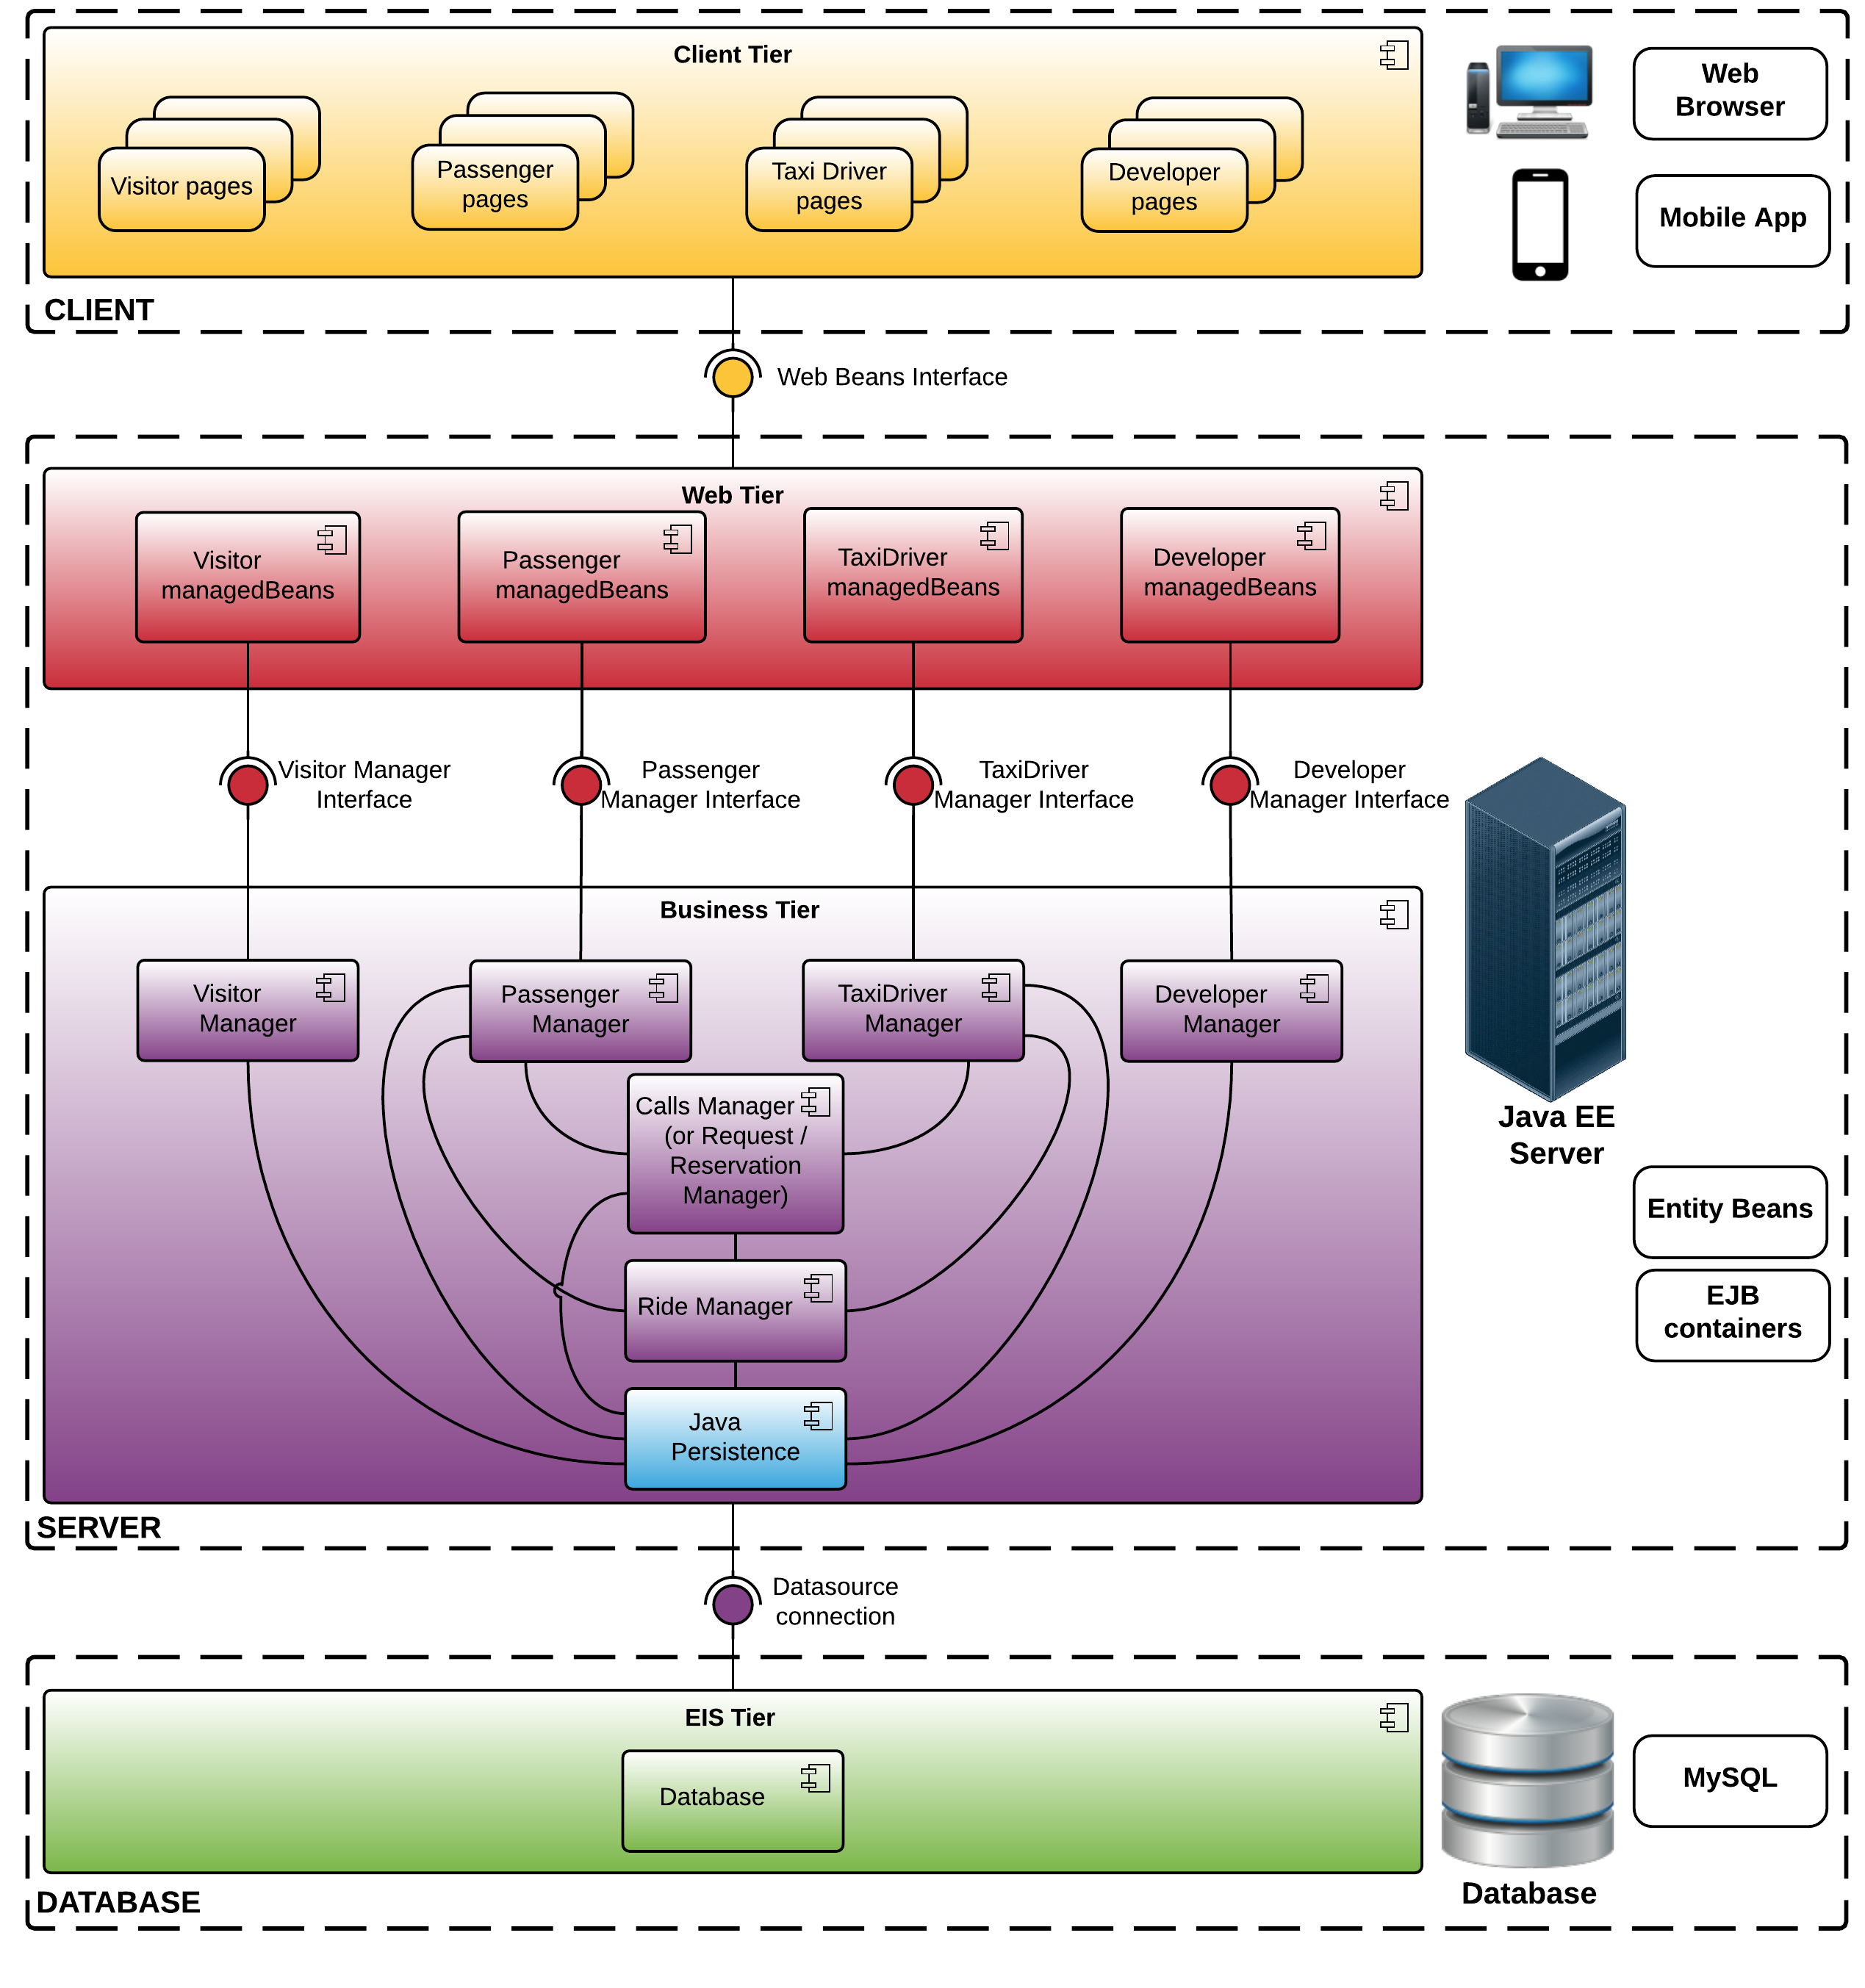
\includegraphics[width=\textwidth]{cpt/img/HighLevelComponentView}
\caption{High Level Components view and their interaction}
\label{fig:HLC}
\end{figure}
\clearpage

\section{Component View}
\subsection{Client Component}
The first component inside the system is the Client component which is responsible of translating user actions and presenting the output of tasks and results into something the user can understand. This component present different interfaces that allows each user to visualize the right pages. Each interface is a subcomponent of the Client components and contains different pages, so different users can visualize different contents with respect to their type.

\begin{figure}[htbp]
\centering
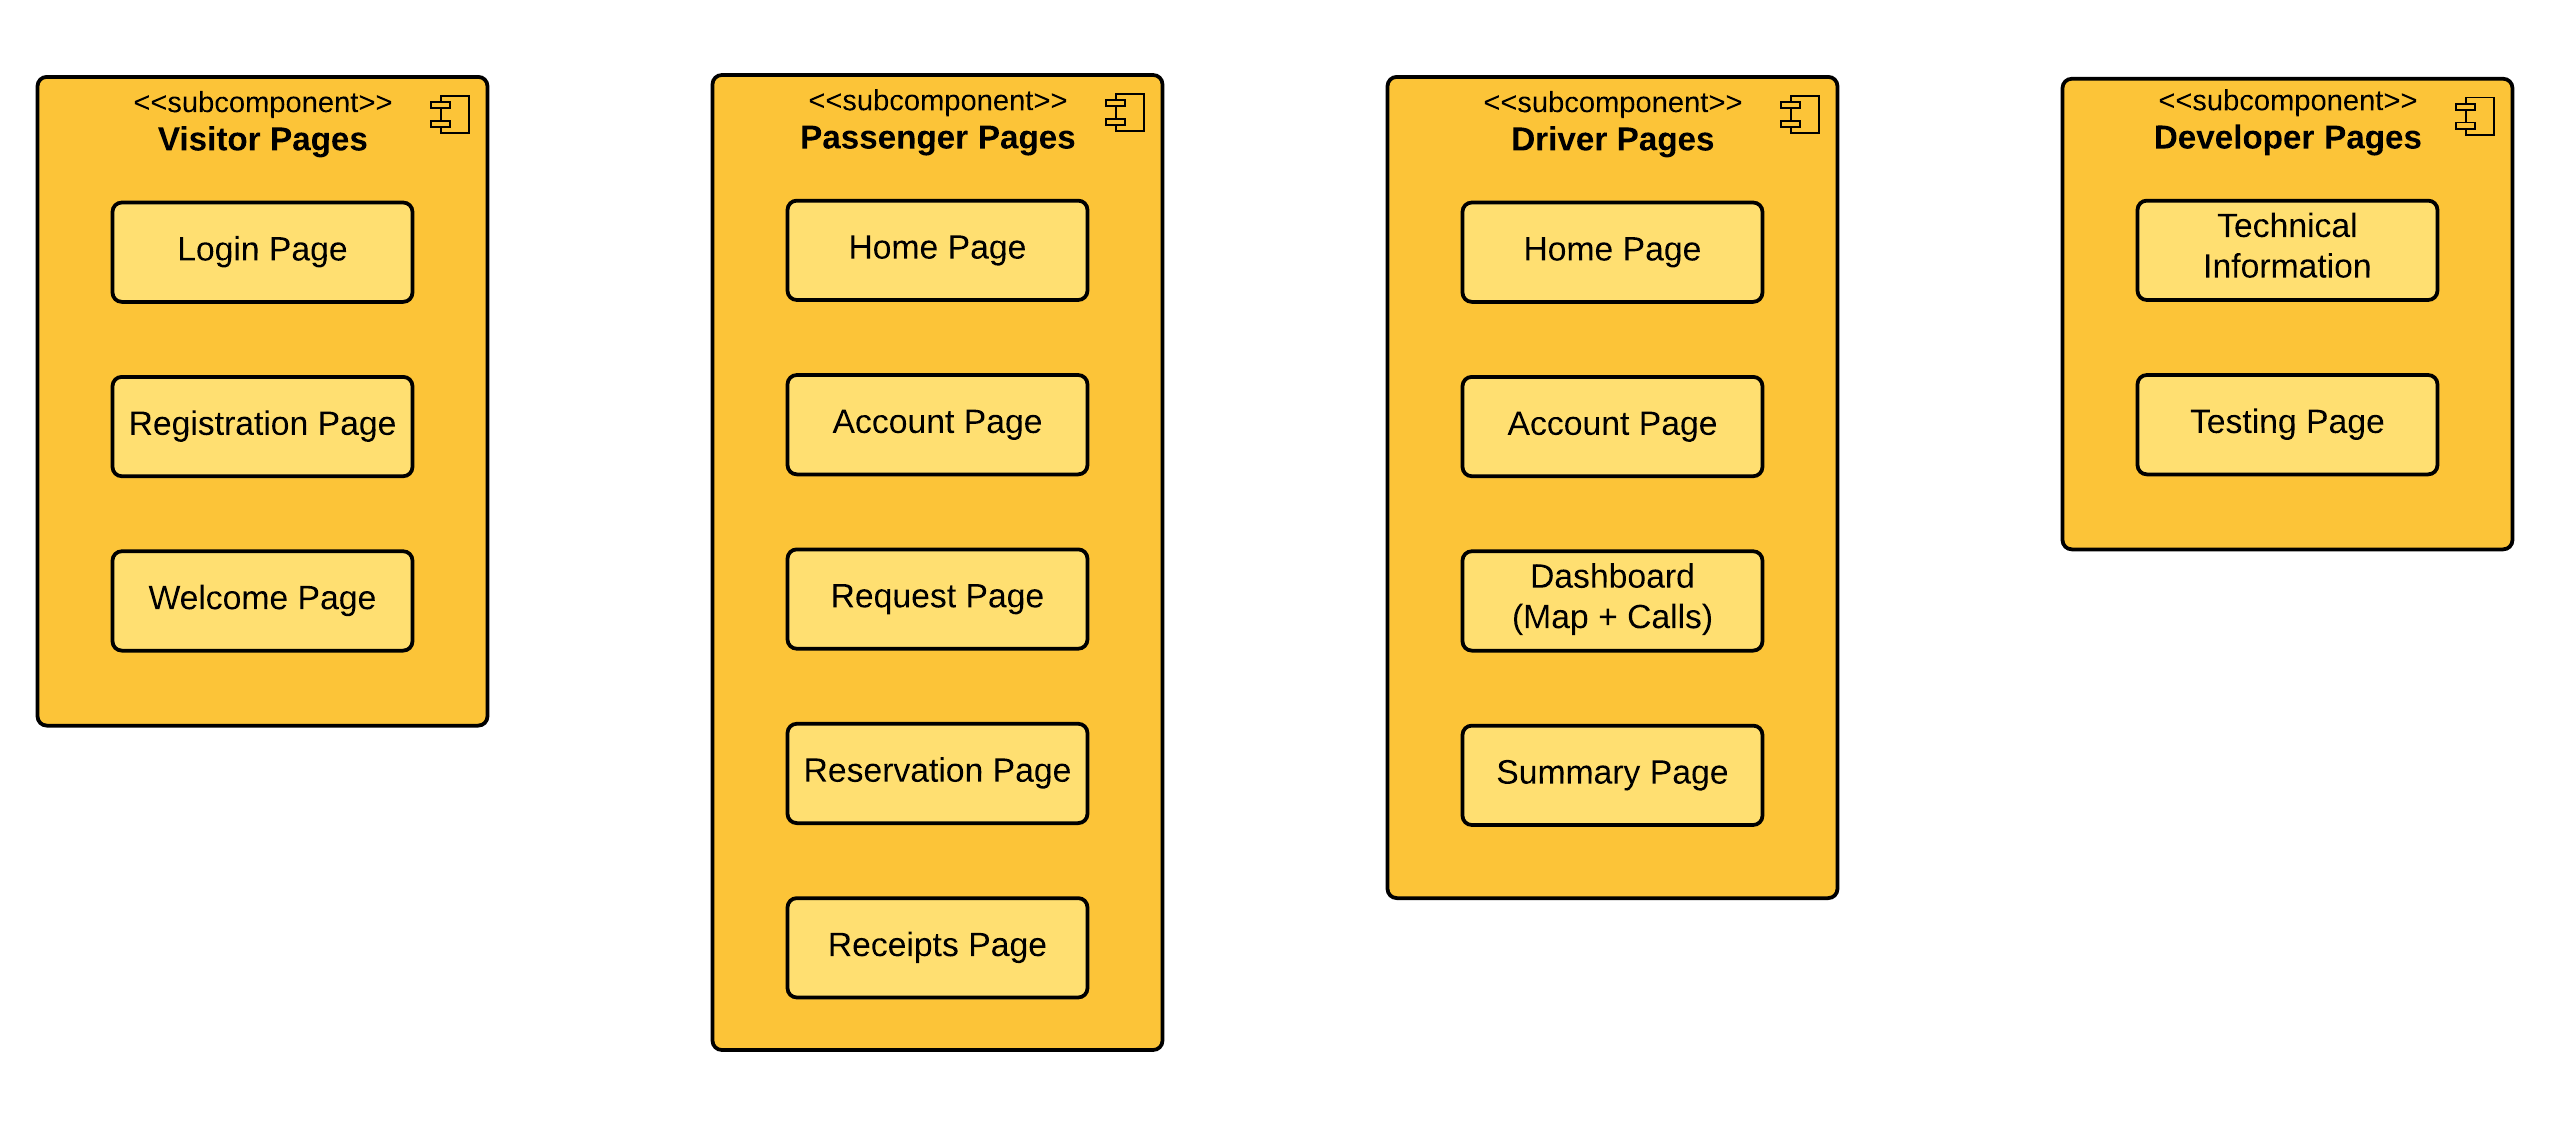
\includegraphics[width=\textwidth]{cpt/img/ClientInterfaces}
\caption{Client subcomponents}
\end{figure}
\clearpage

\subsection{Web Component}
The Web component generates dynamic web pages containing XHTML.
Web components implements Java Server Faces technology, which is a common  user interface component framework for web applications. In this way every user input in all the client pages is managed by these beans, one per each group of pages. 

\begin{figure}[htbp]
\centering
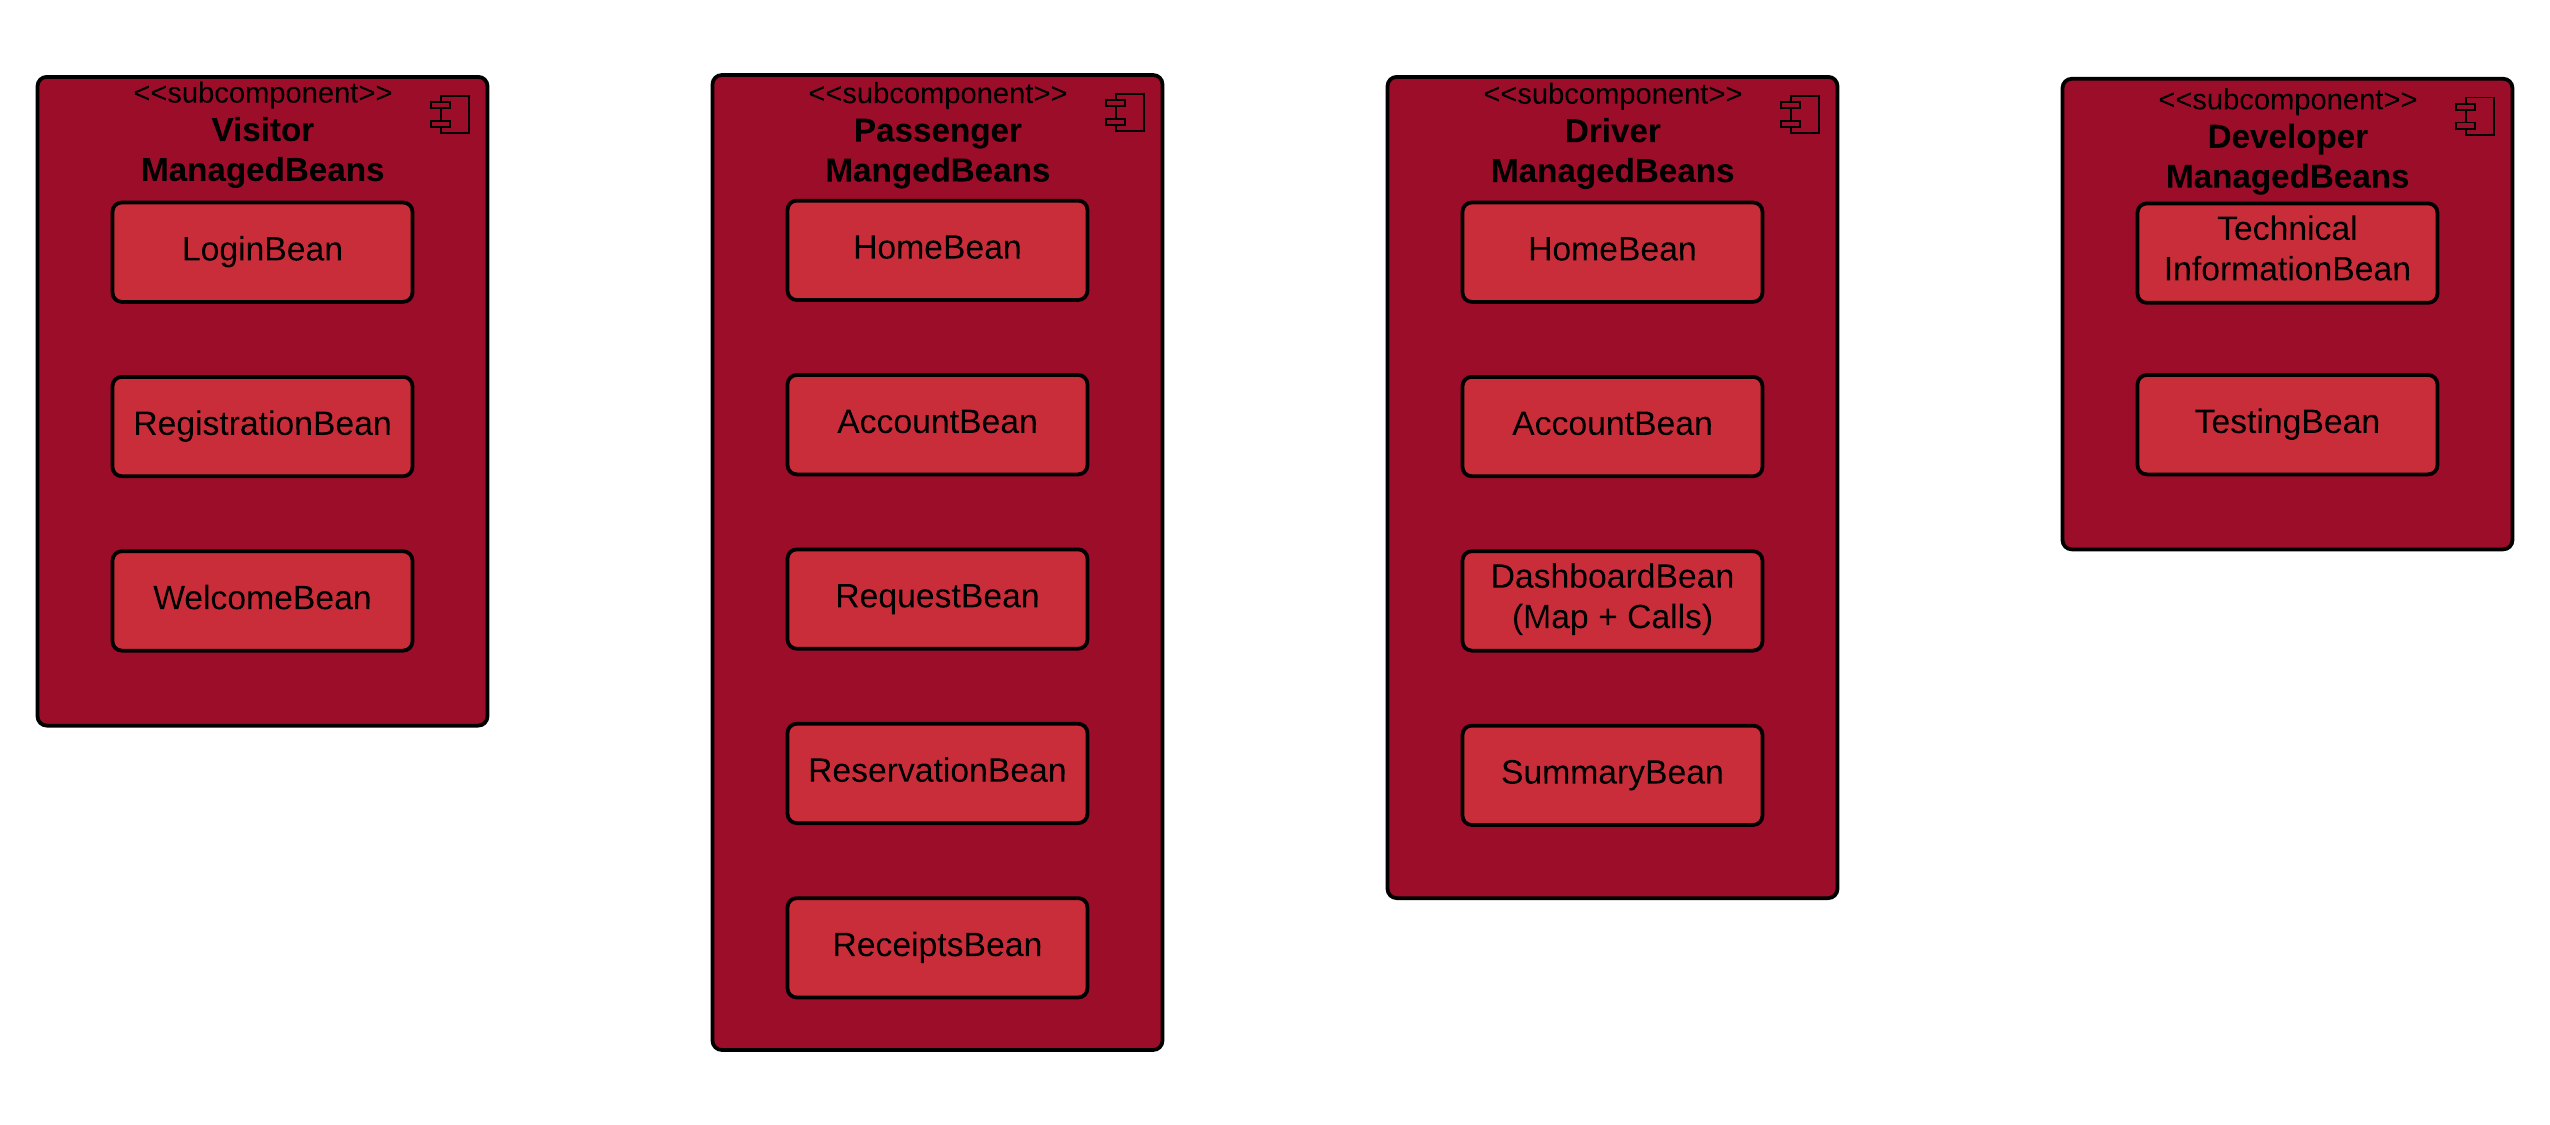
\includegraphics[width=\textwidth]{cpt/img/WebInterfaces}
\caption{Web subcomponents}
\end{figure}
\clearpage

\subsection{Business Logic Component}
The Business Logic component coordinates the application, processes commands, makes logical decisions and evaluations, and performs calculations. It also moves and processes data between the Client and the Java Persistence Entity, which holds the information of the system data model, and is in charge of storing and retrieving information from a database.
In this first release of the Design Document we have focused only on a small number of fundamental elements (Java Beans) necessary to manage the basic functionalities offered to the users by the system. Further additions will be necessary during the development.
More in detail:
\begin{itemize}
	\item Visitor Manager $\rightarrow$ Offers functionalities to:
	\begin{itemize}
		\item Check the validity and correctness of the information provided by the user 
		\item Create new users and save them into the system;
		\item Check if the Login is valid and authenticate users;
		\item Trigger the right user manager depending on the type of user that has logged in.
	\end{itemize}
	\item Passenger Manager $\rightarrow$ Manages the passenger requests (taxi requests, reservations), the passenger profile and his status.
	\item Taxi Driver Manager $\rightarrow$ Manages all the operations made by taxi drivers, like accepting or rejecting incoming calls or ending rides.
	\item Developer Manager $\rightarrow$ Manage all the operations made by developers (add new features, update the system code and architecture).
	\item Ride Manager $\rightarrow$ Offers functionalities to:
	\begin{itemize}
		\item Create and manage the route for the ride;
		\item Keep track of the passengers and the driver involved in the ride, and all the information: duration, distance, fee, route for the entire ride and for each passenger.
	\end{itemize}
	\item Call Manager $\rightarrow$ Manages all the passenger's requests/reservations, the taxi queue for every area and the matching for show rides.
\end{itemize}

\begin{figure}[htbp]
\centering
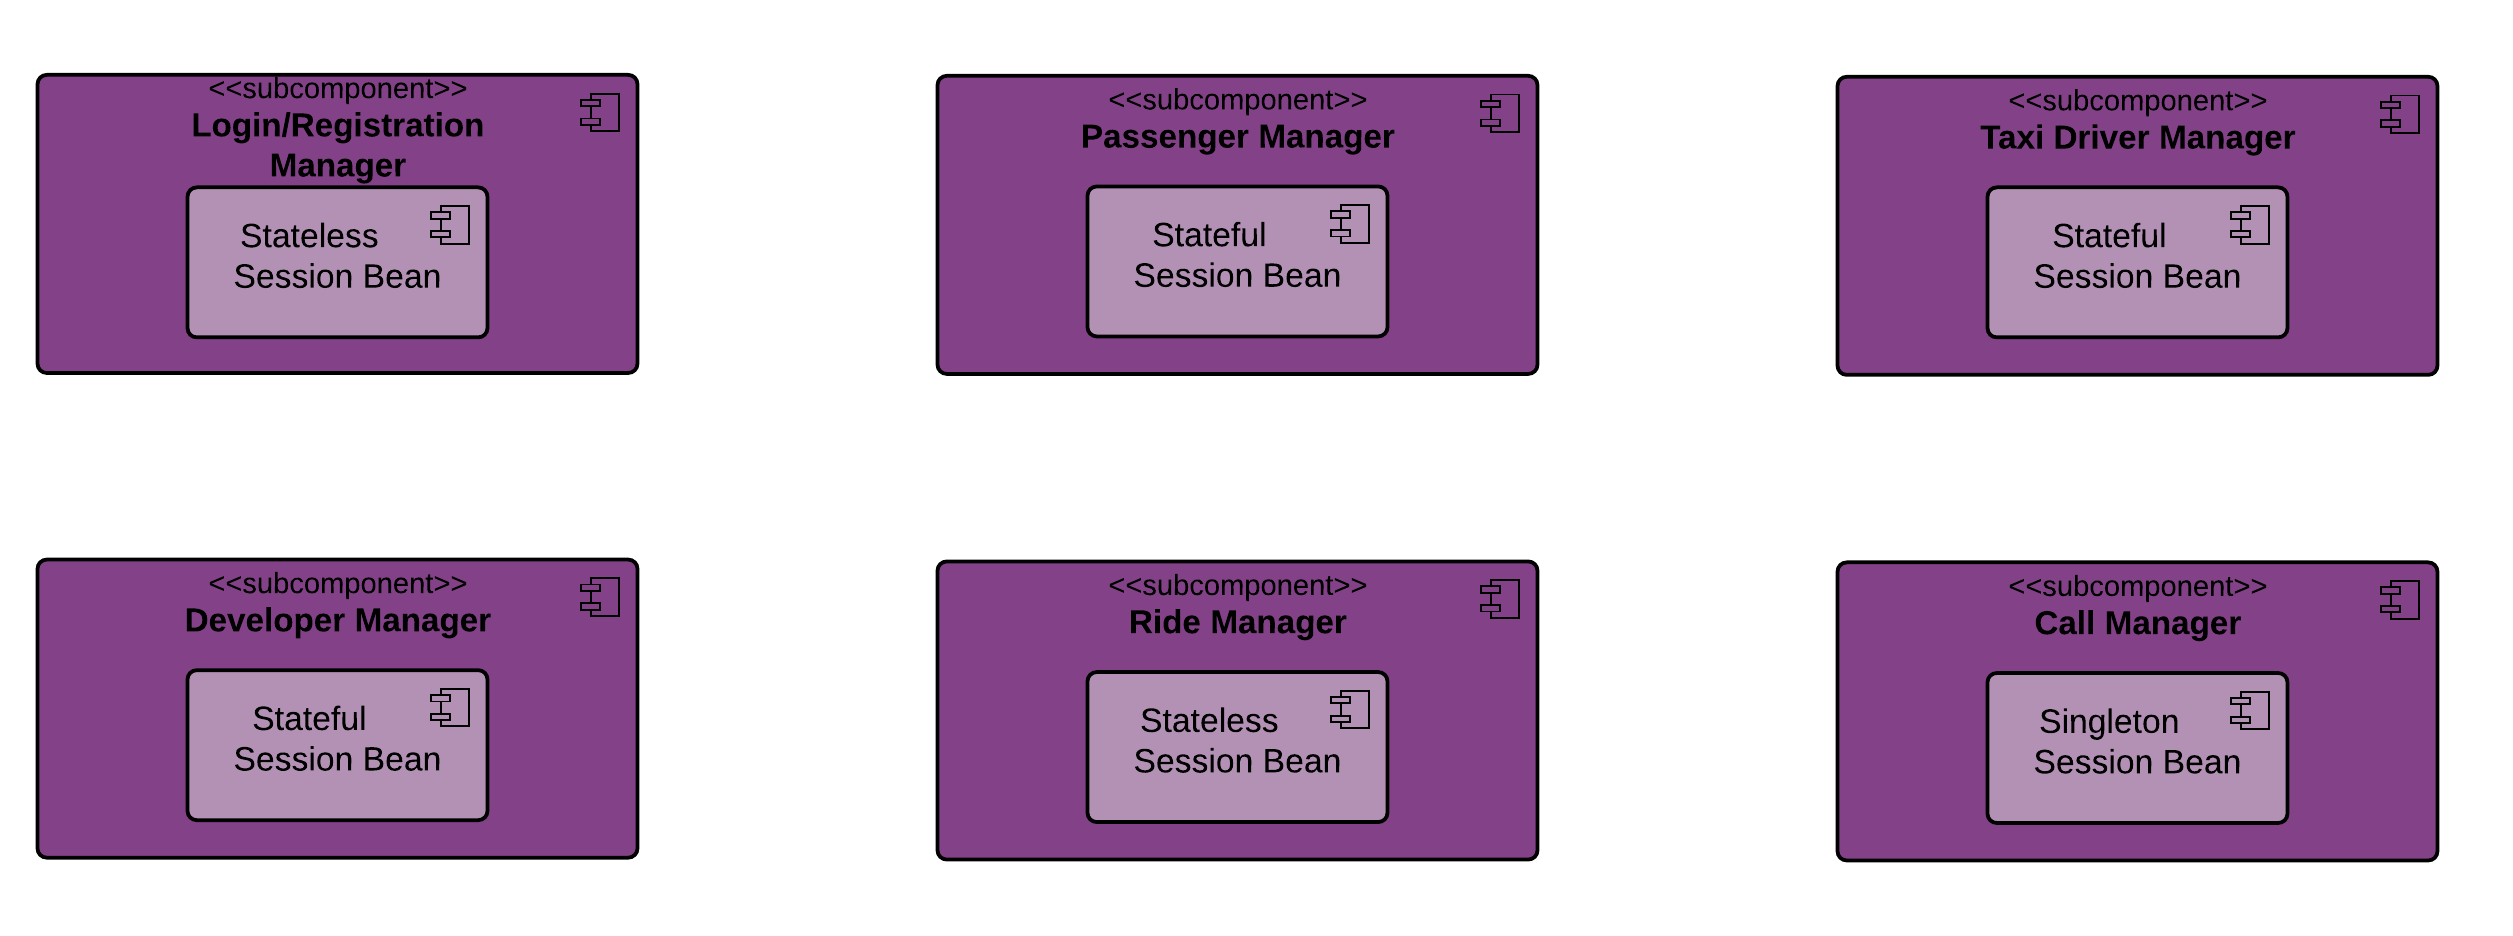
\includegraphics[width=\textwidth]{cpt/img/ServerInterfaces}
\caption{Business Logic subcomponents}
\end{figure}
\clearpage

\subsection{Database Component}
The conceptual architecture of the database is depicted in this diagram using the notation of Entity - Relation Diagram which is useful to individuate all the entities of the system and their mutual relationship.

\begin{figure}[htbp]
\centering
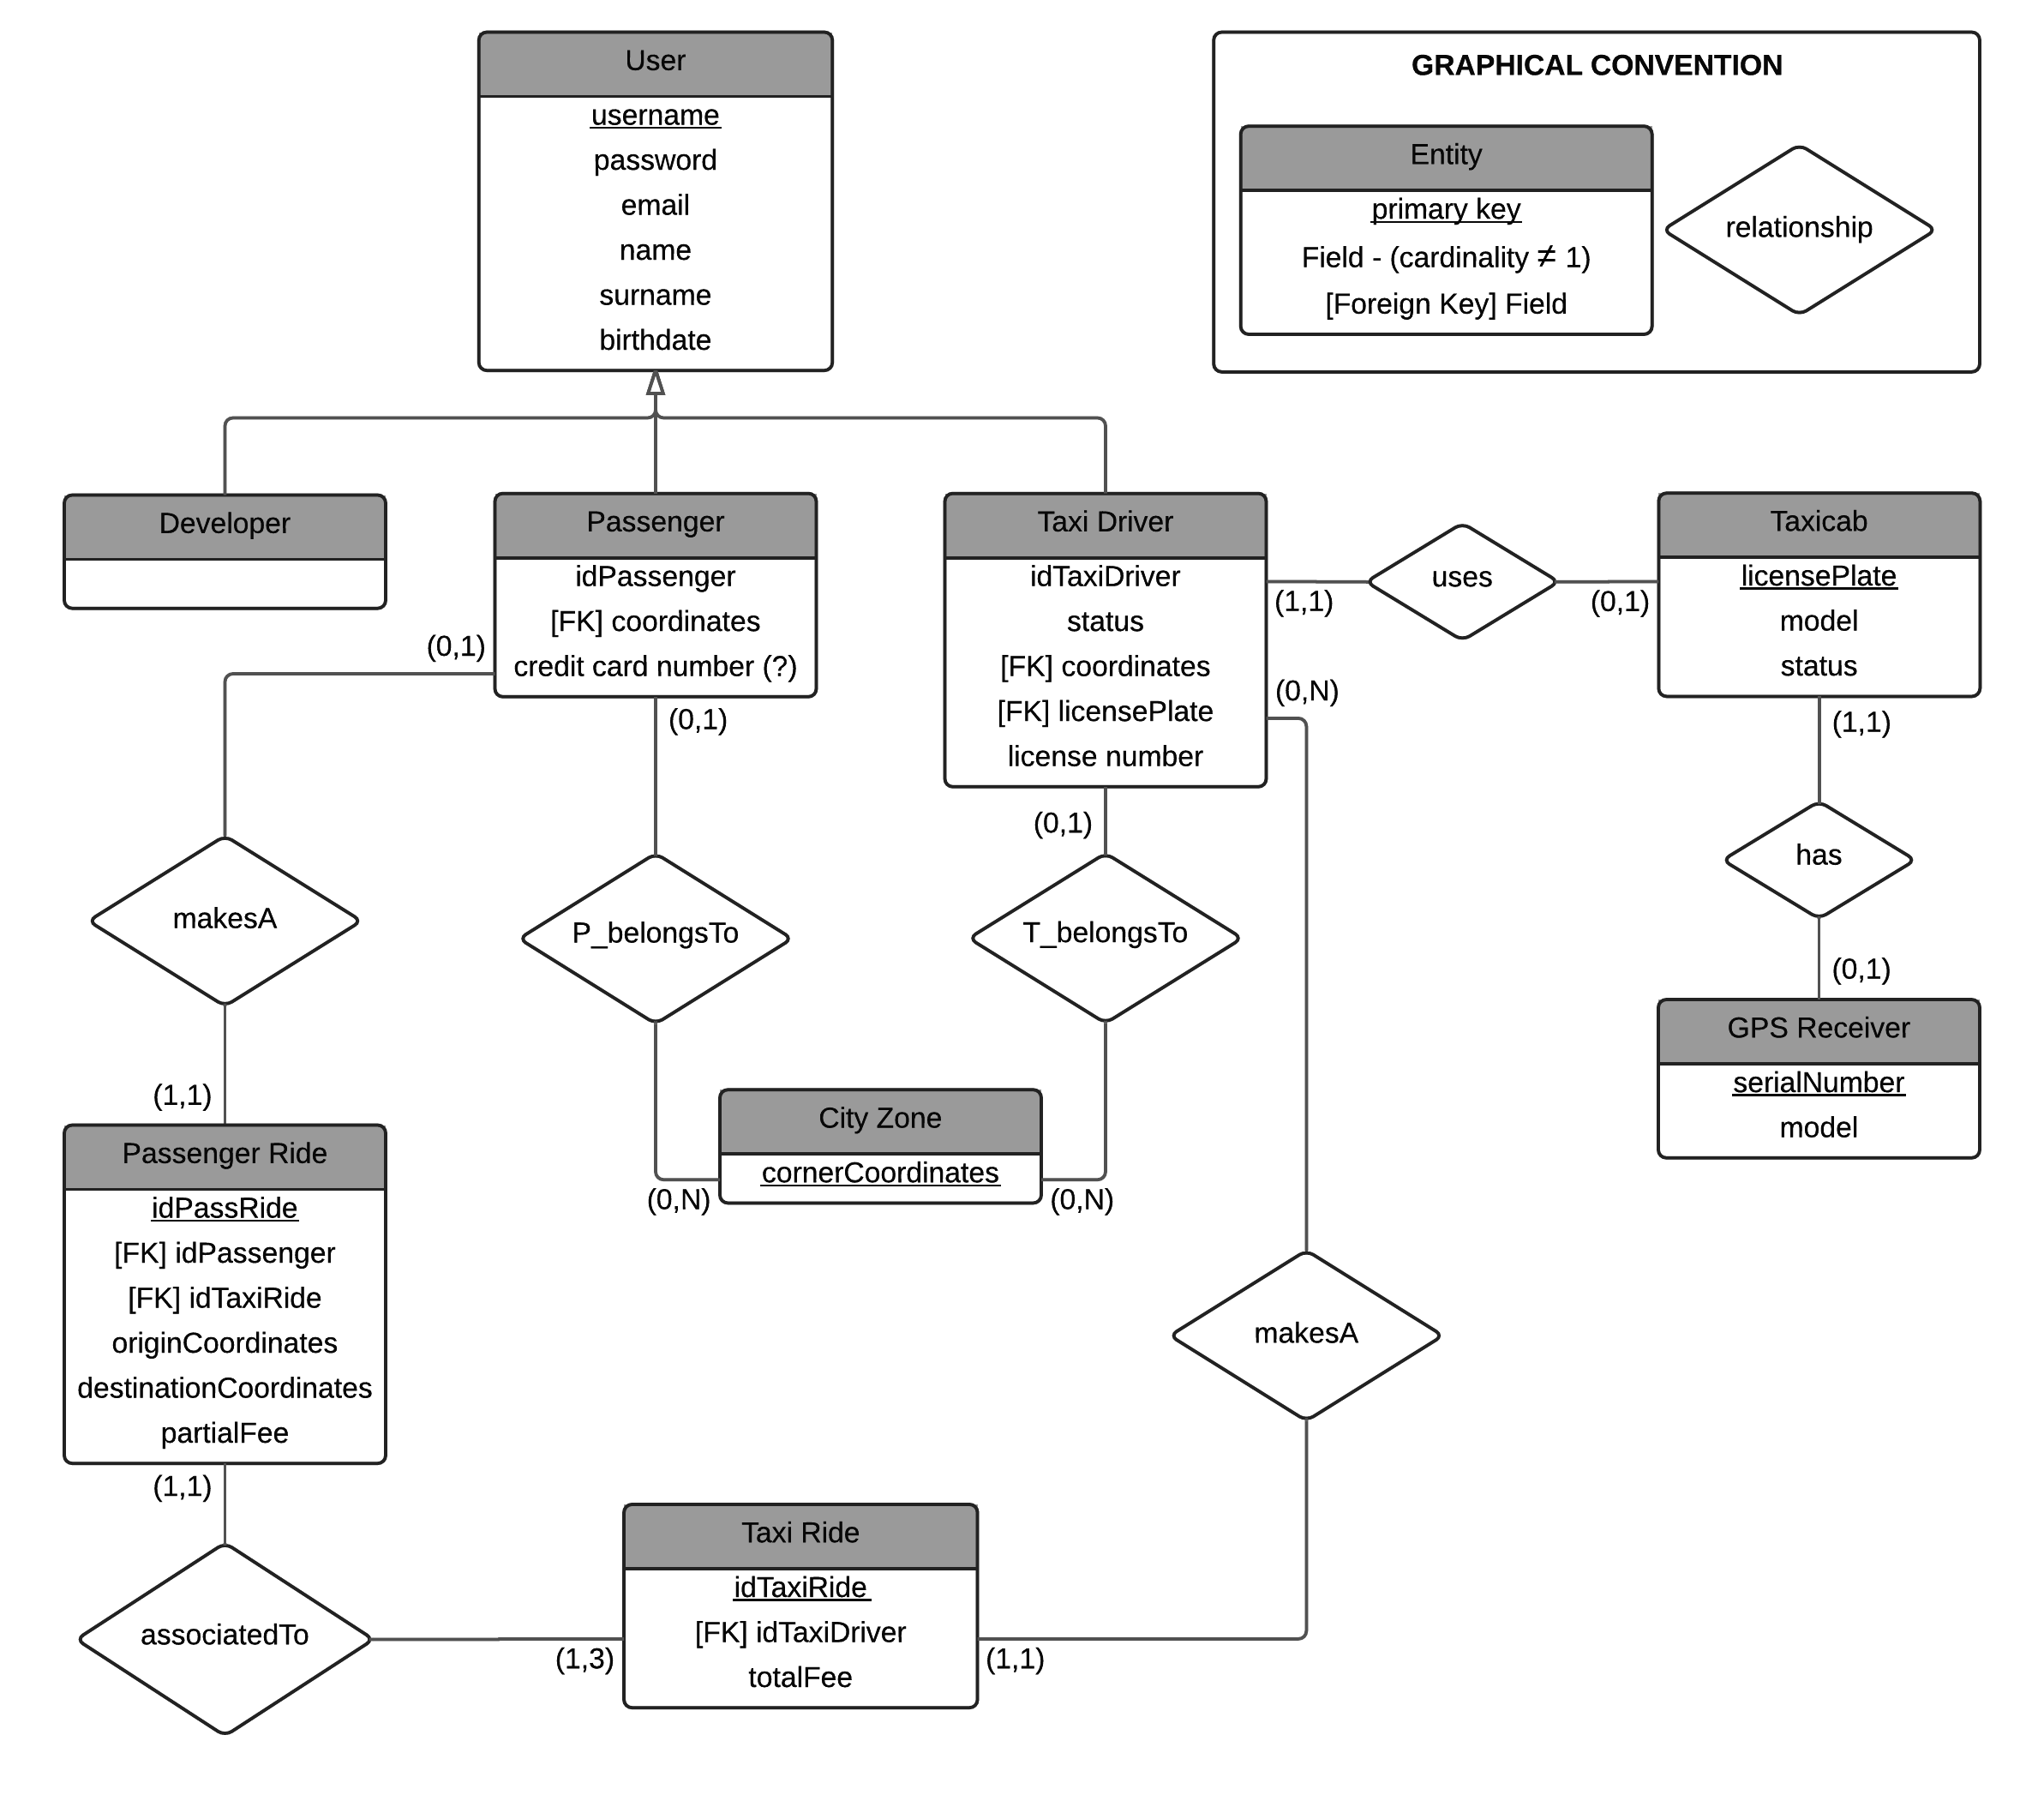
\includegraphics[width=\textwidth]{cpt/img/Database}
\caption{Database ER Diagram}
\end{figure}
\clearpage

\section{Deployment View}
The diagram in Figure \ref{fig:Deploy} shows the deployment view of the software product. Because of the early stage of the developing of the system, this diagram is deliberately simple and only depicts the distinction between client machines, server machines and database machines at large. Further revisions will go deeper into the hardware architecture of the system and will identify more specific hardware components in which the software will be deployed.

\begin{figure}[htbp]
\centering
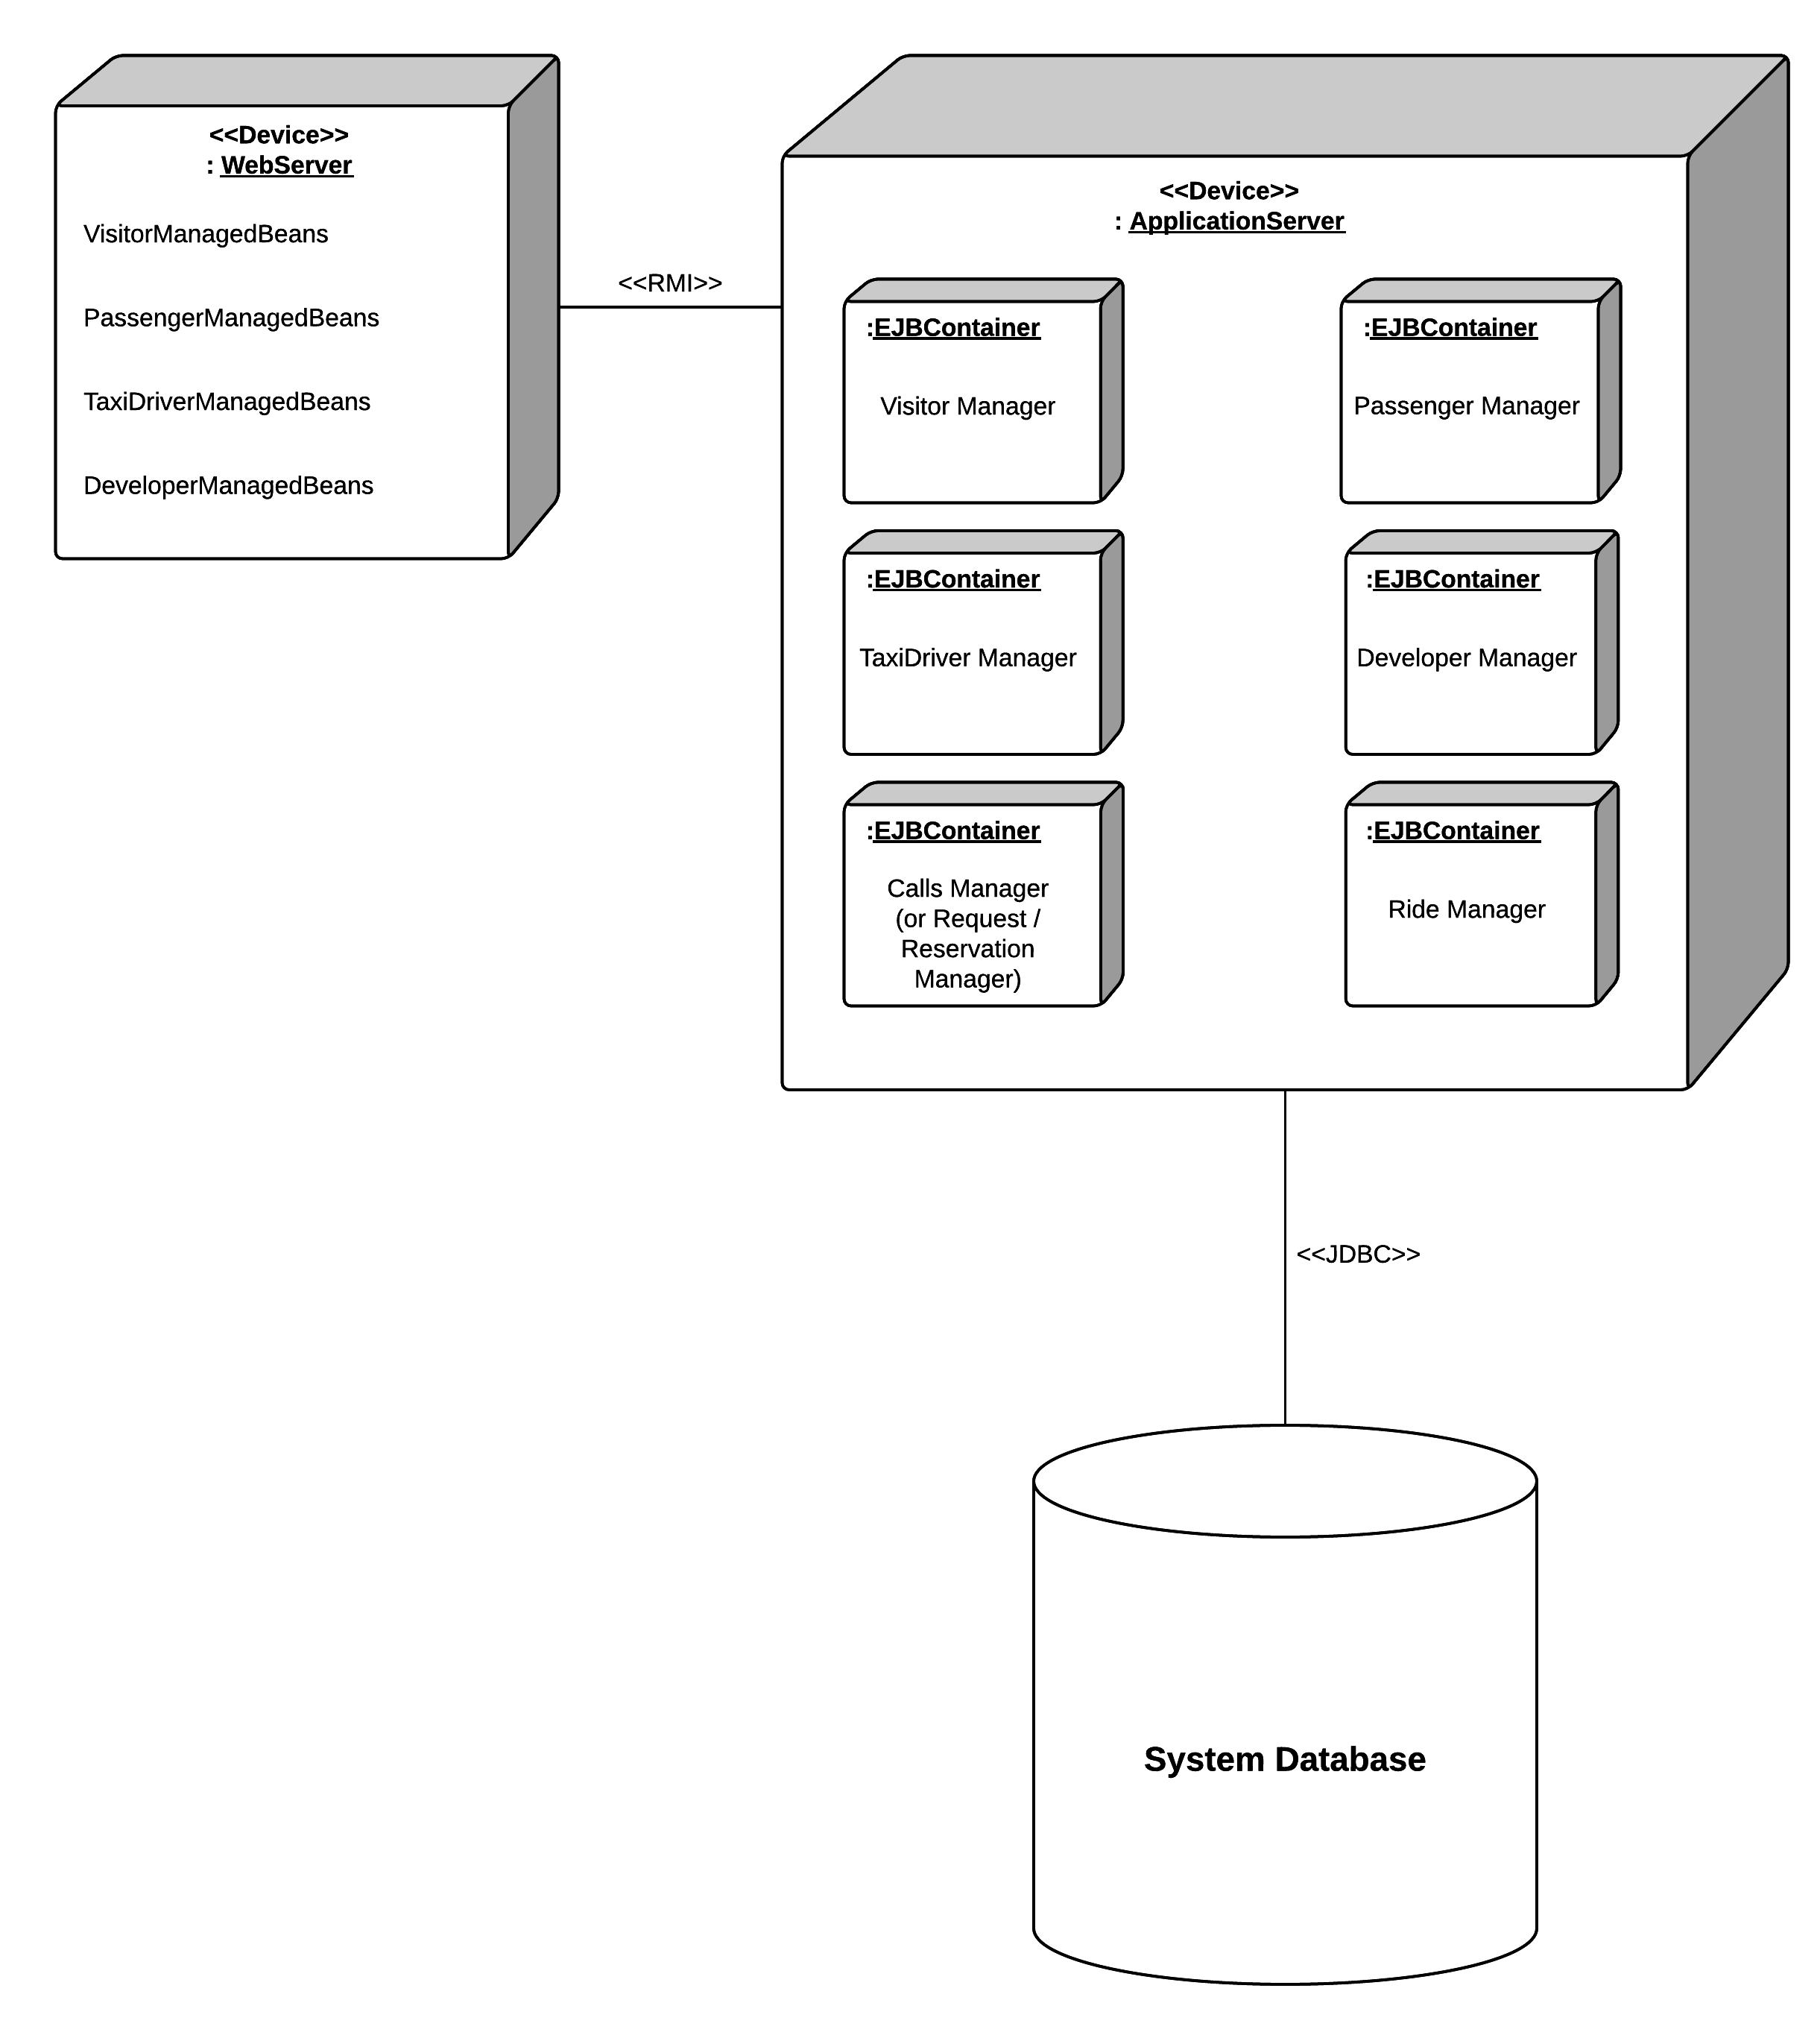
\includegraphics[width=\textwidth]{cpt/img/RuntimeDeploymentView}
\caption{Deployment view}
\label{fig:Deploy}
\end{figure}
\clearpage

\section{Runtime View}
The following diagrams depicts the runtime view of MyTaxiService project describing in a simple way how the various components defined until this point behave in order to accomplish some of the most important activities of the system.

\begin{itemize}
	\item This diagram represents the components that are involved in the taxi request and reservation activities, and their interaction
	\begin{figure}[htbp]
	\centering
	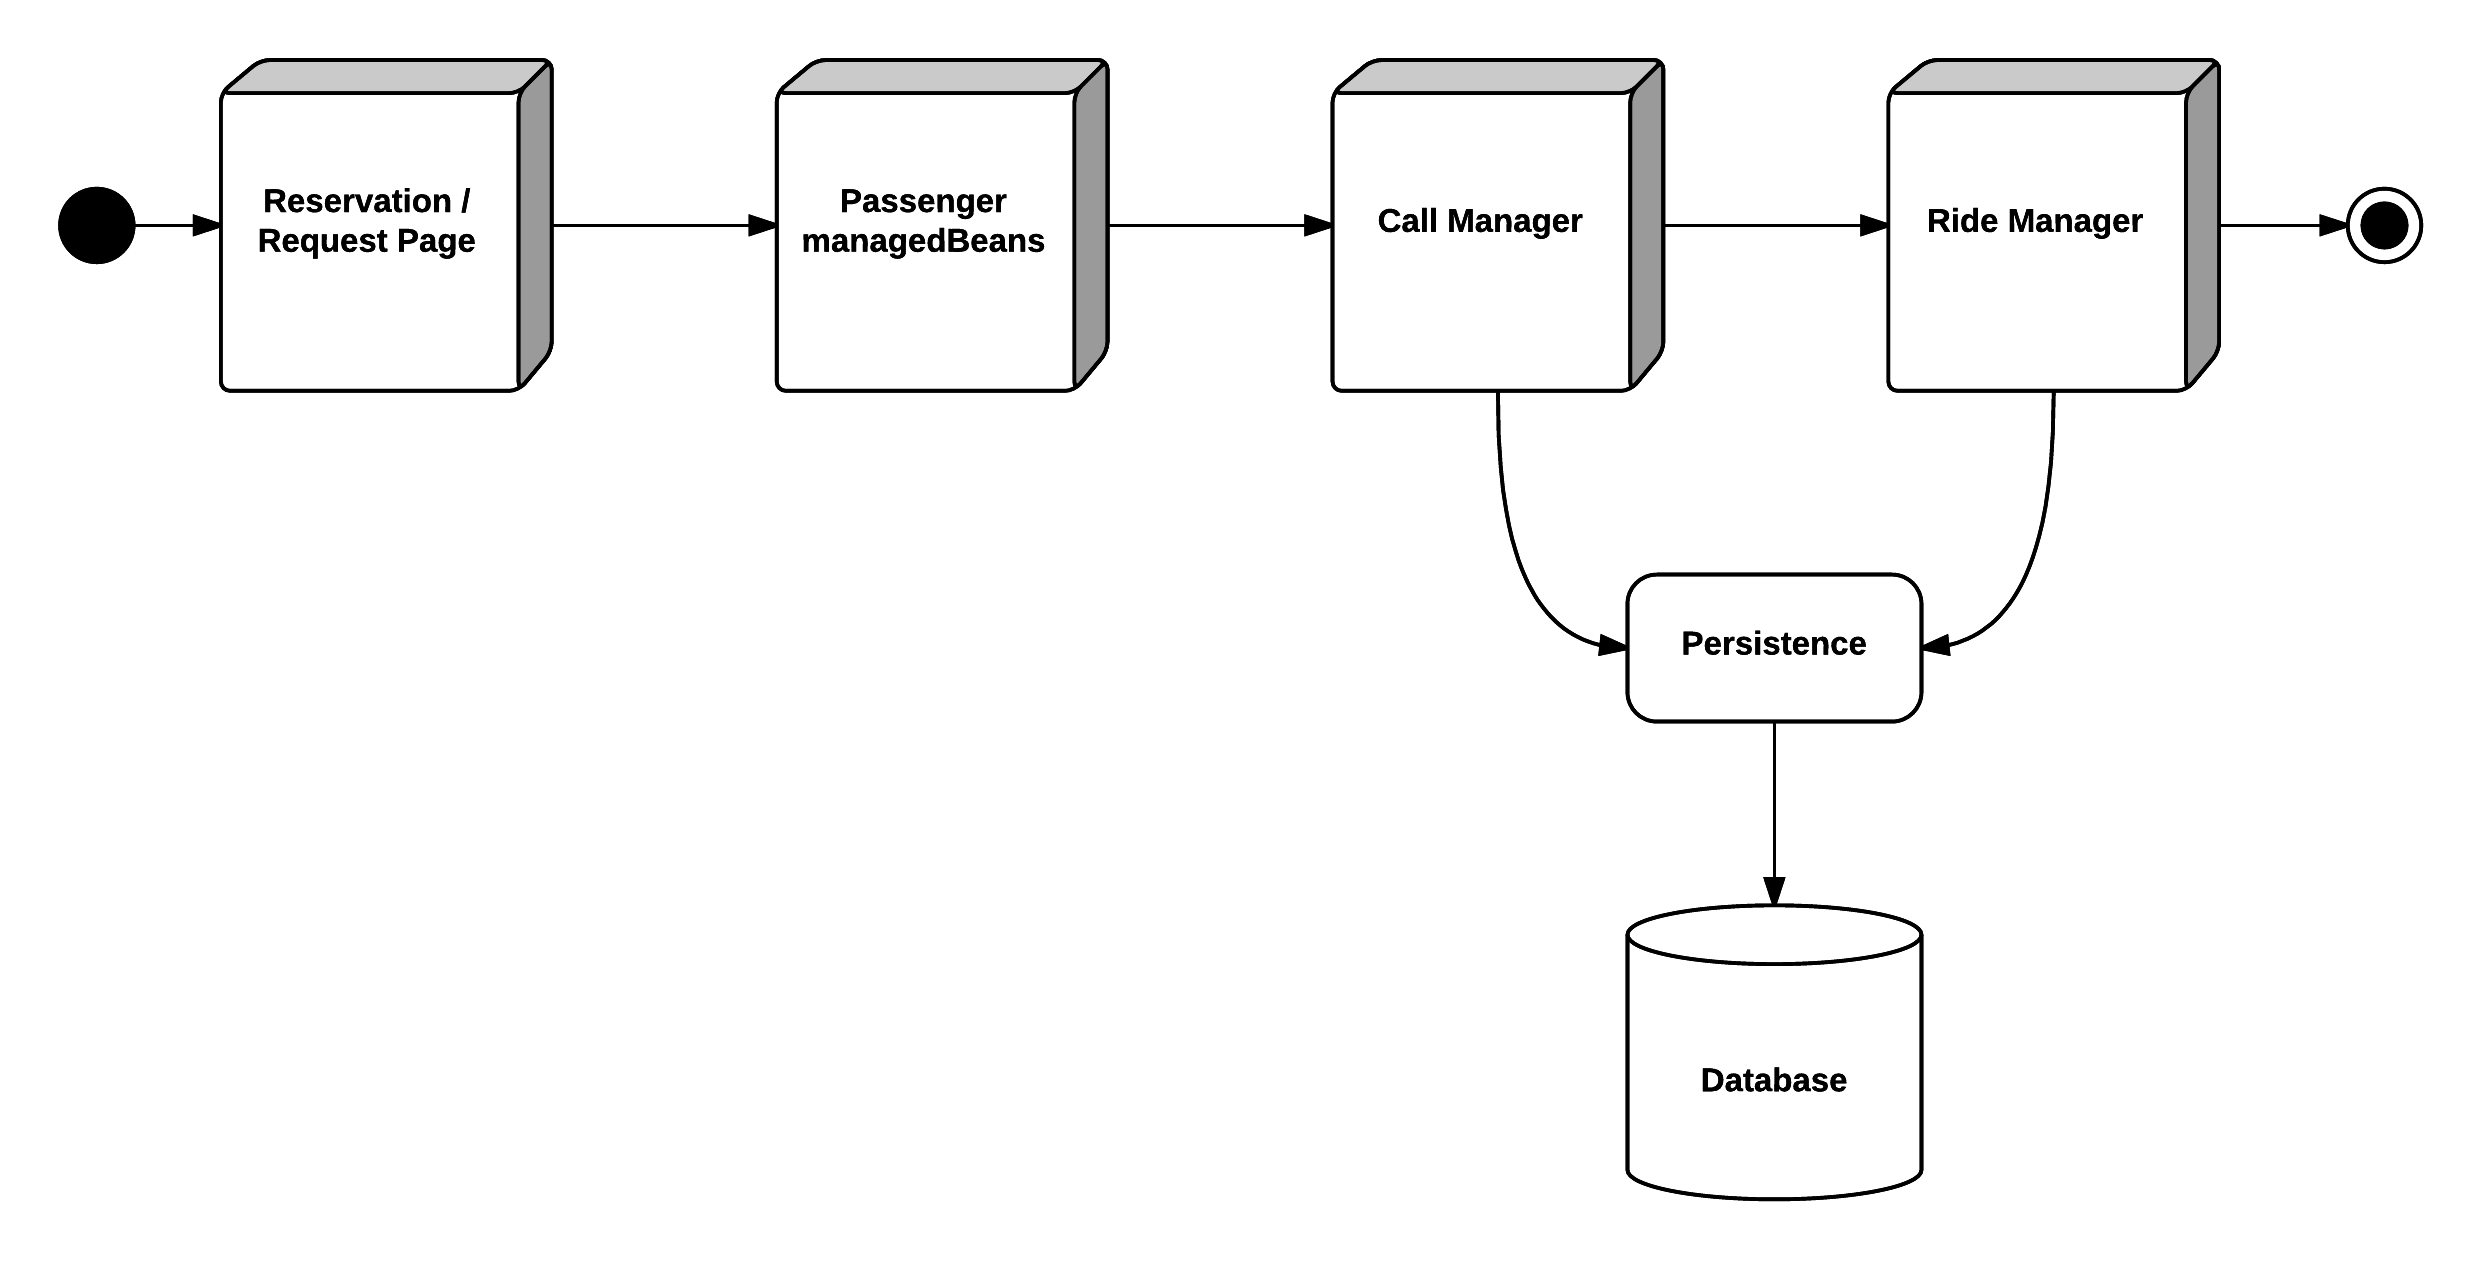
\includegraphics[width=\textwidth]{cpt/img/RuntimeReqResView}
	\caption{Runtime Taxi Request and Reservation}
	\end{figure}
	\clearpage
	
	\item This diagram represents the activity of showing the receipts to the user
	\begin{figure}[htbp]
	\centering
	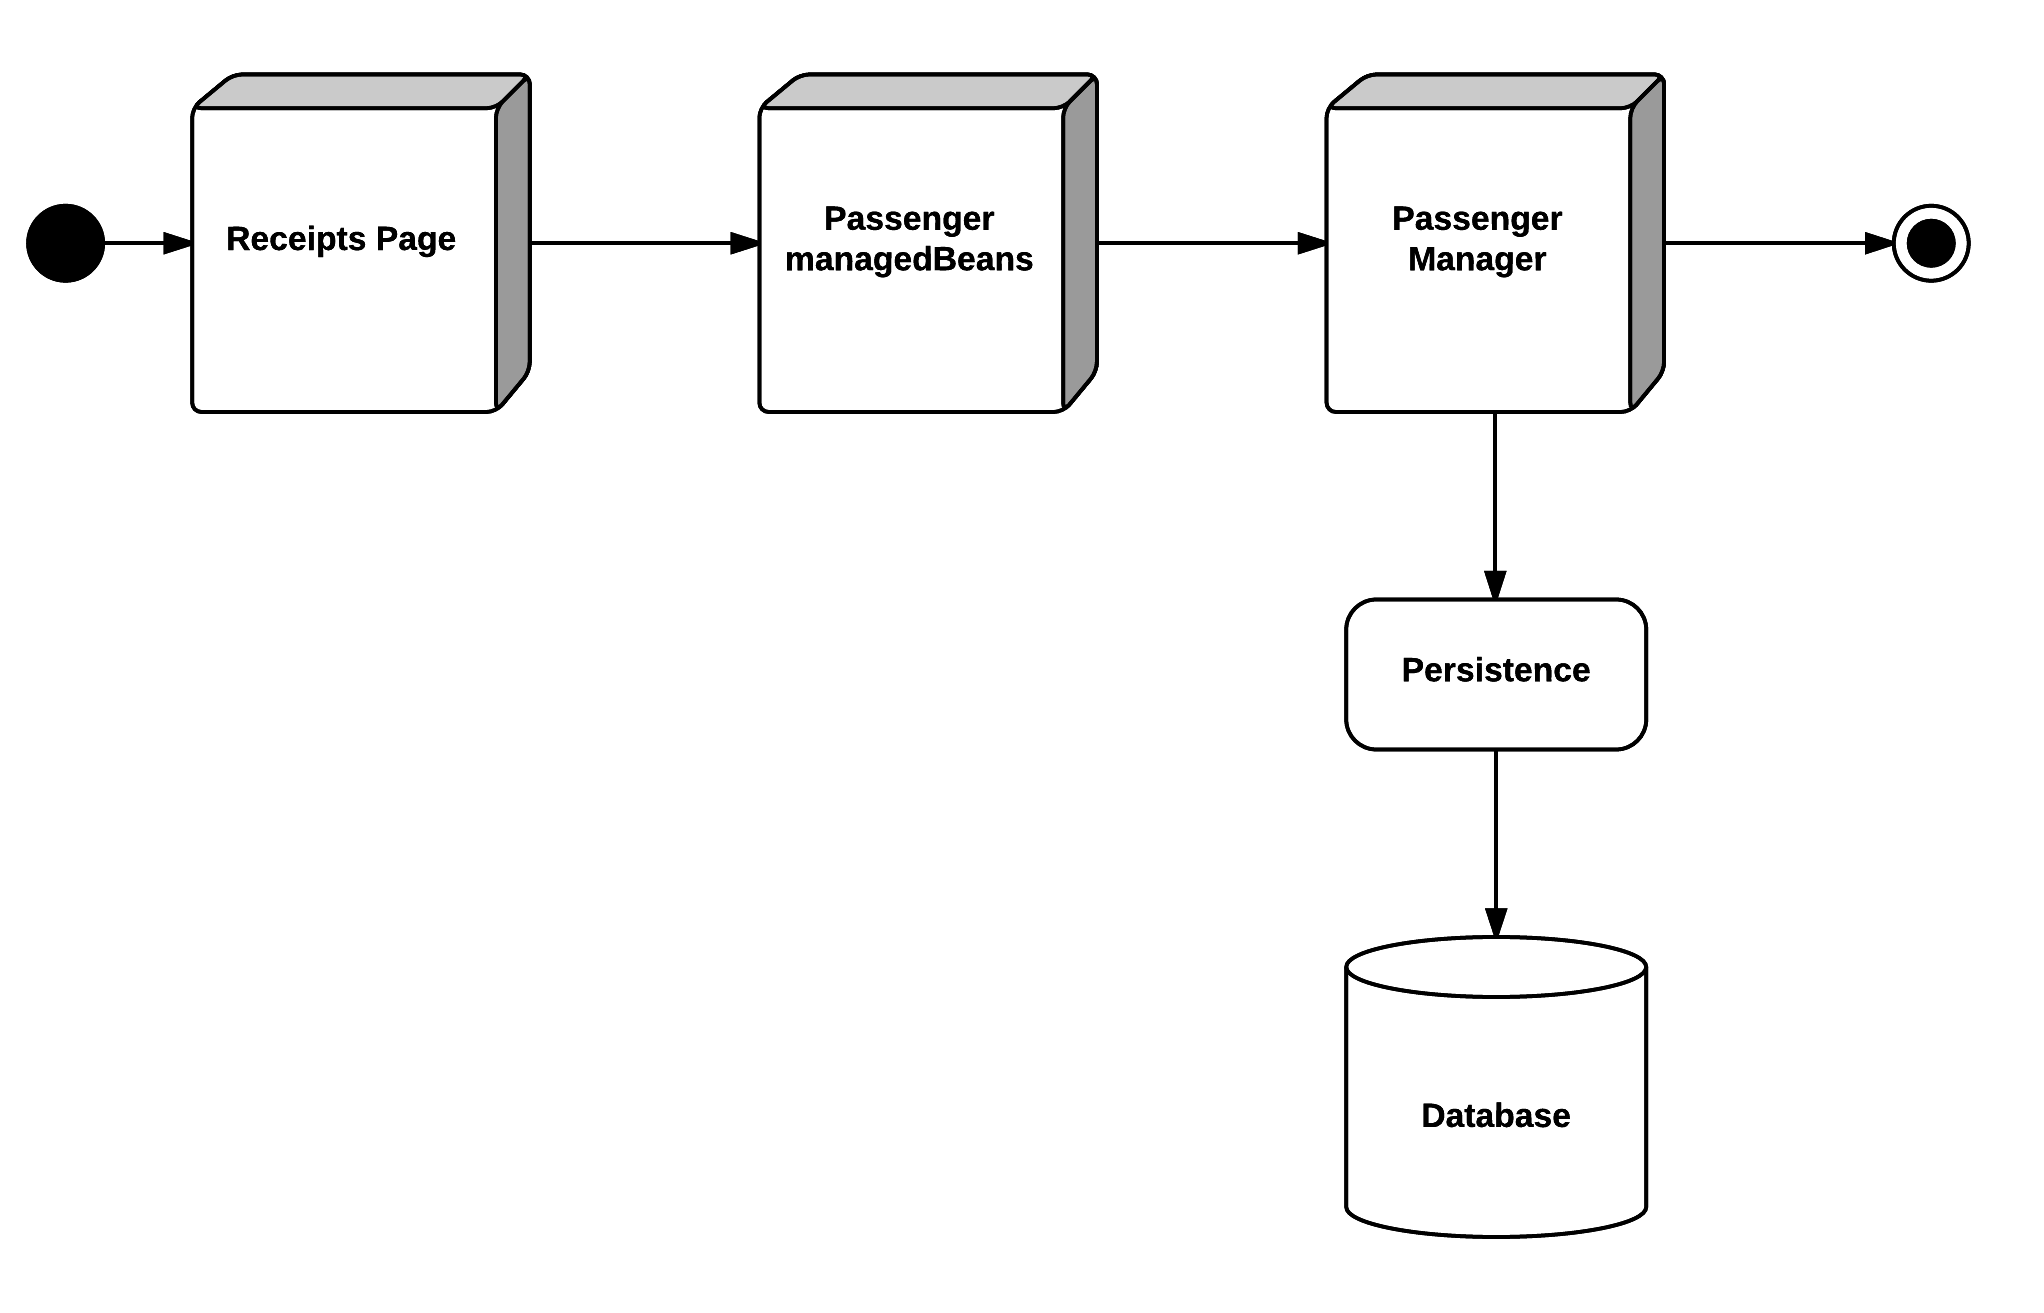
\includegraphics[width=\textwidth]{cpt/img/RuntimeReceiptsView}
	\caption{Runtime get receipts}
	\end{figure}
	\clearpage
	
	\item This diagram represents the components that are involved in the modification of the passenger?s account, and their interaction
	\begin{figure}[htbp]
	\centering
	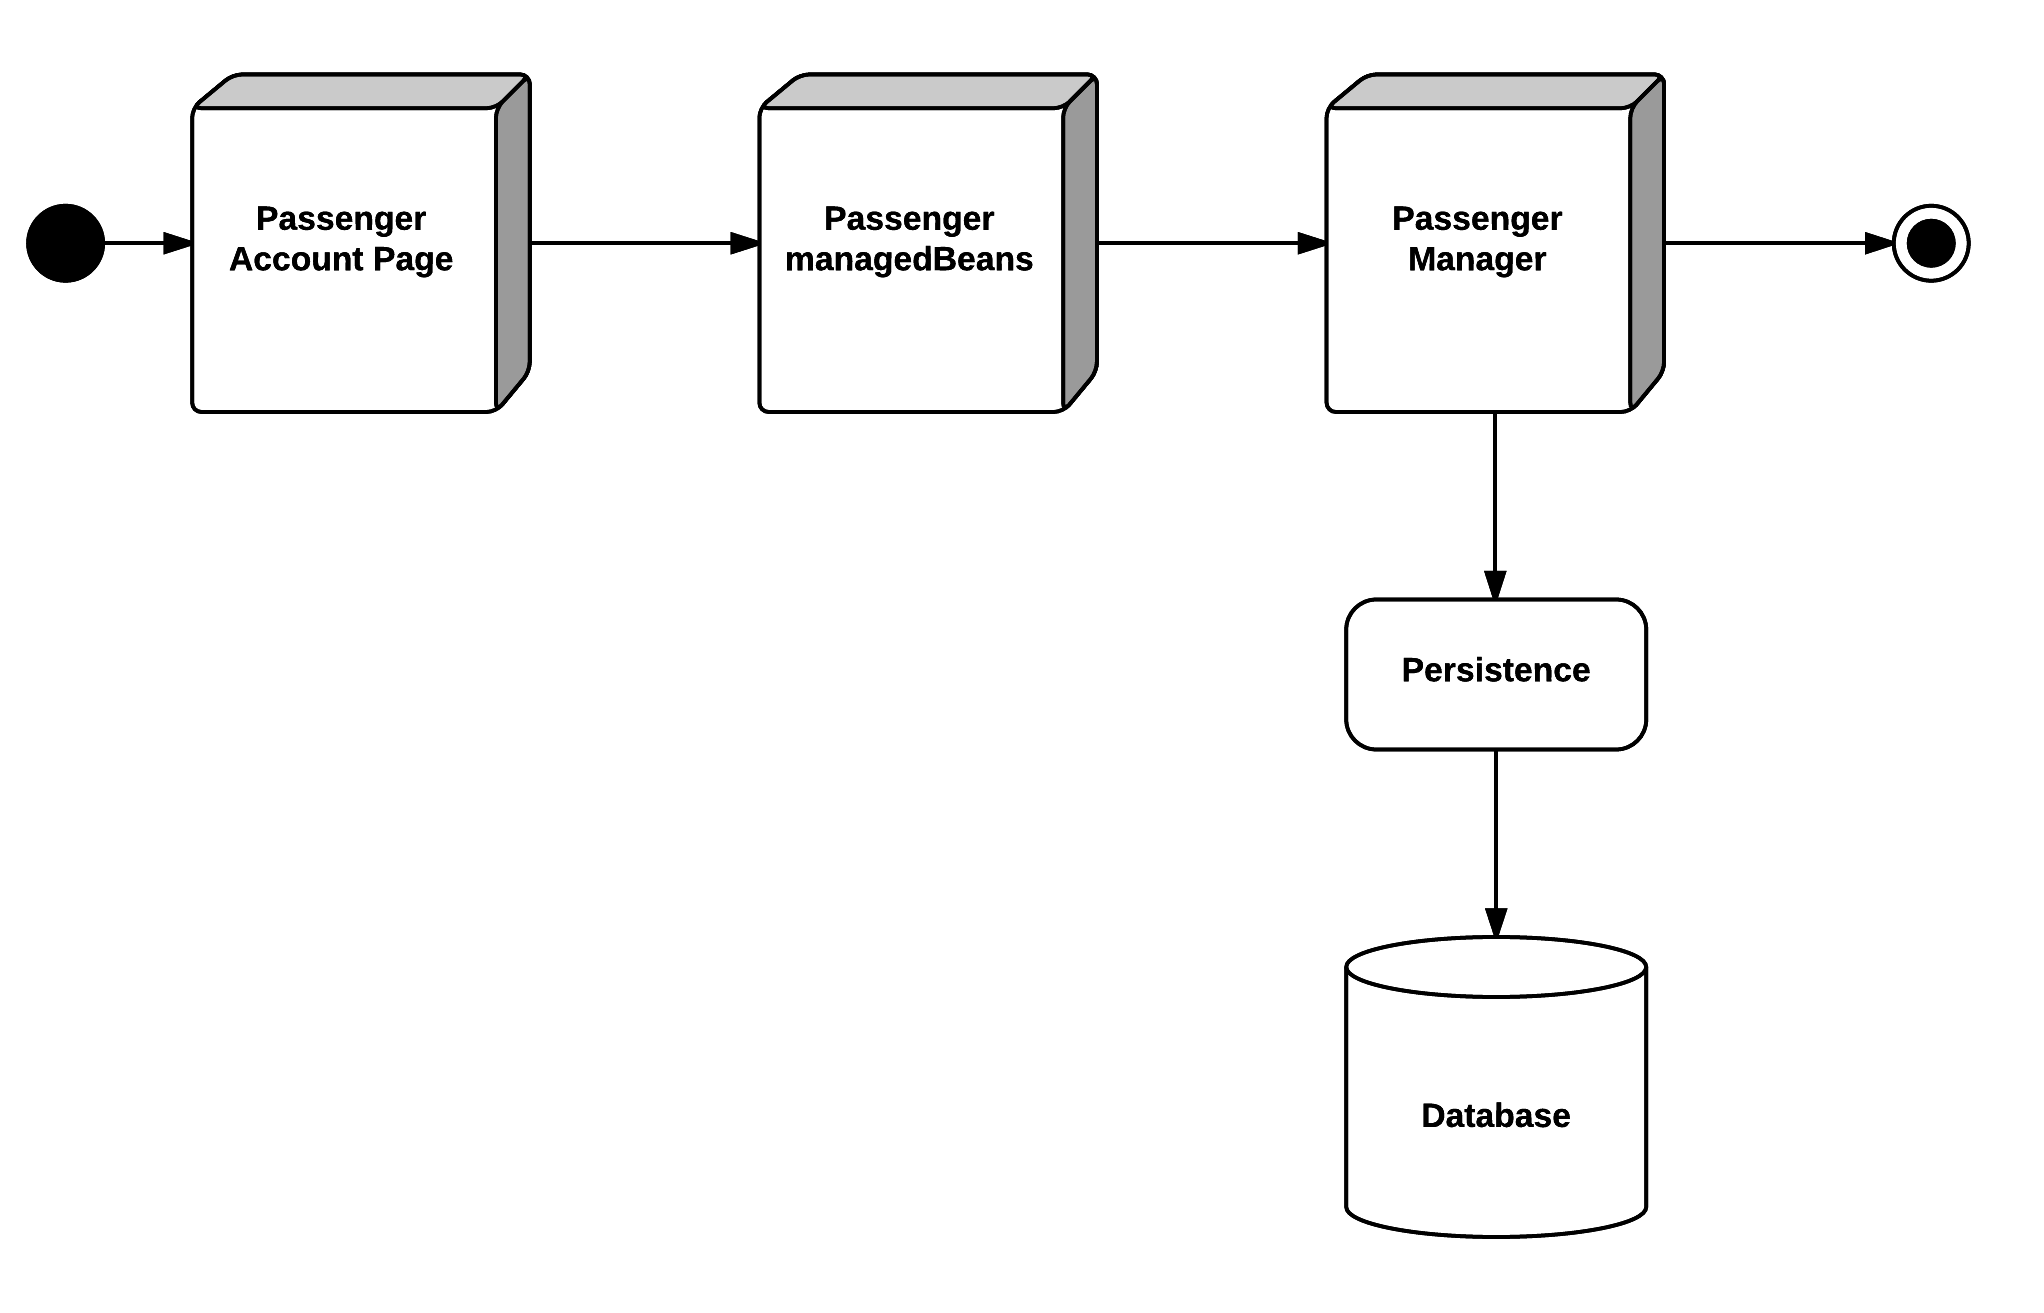
\includegraphics[width=\textwidth]{cpt/img/RuntimeModifyPageView}
	\caption{Runtime Modify Passenger's Account}
	\end{figure}
	\clearpage
	
	\item This diagram represents the activity done by the system to let a taxi driver modify his account
	\begin{figure}[htbp]
	\centering
	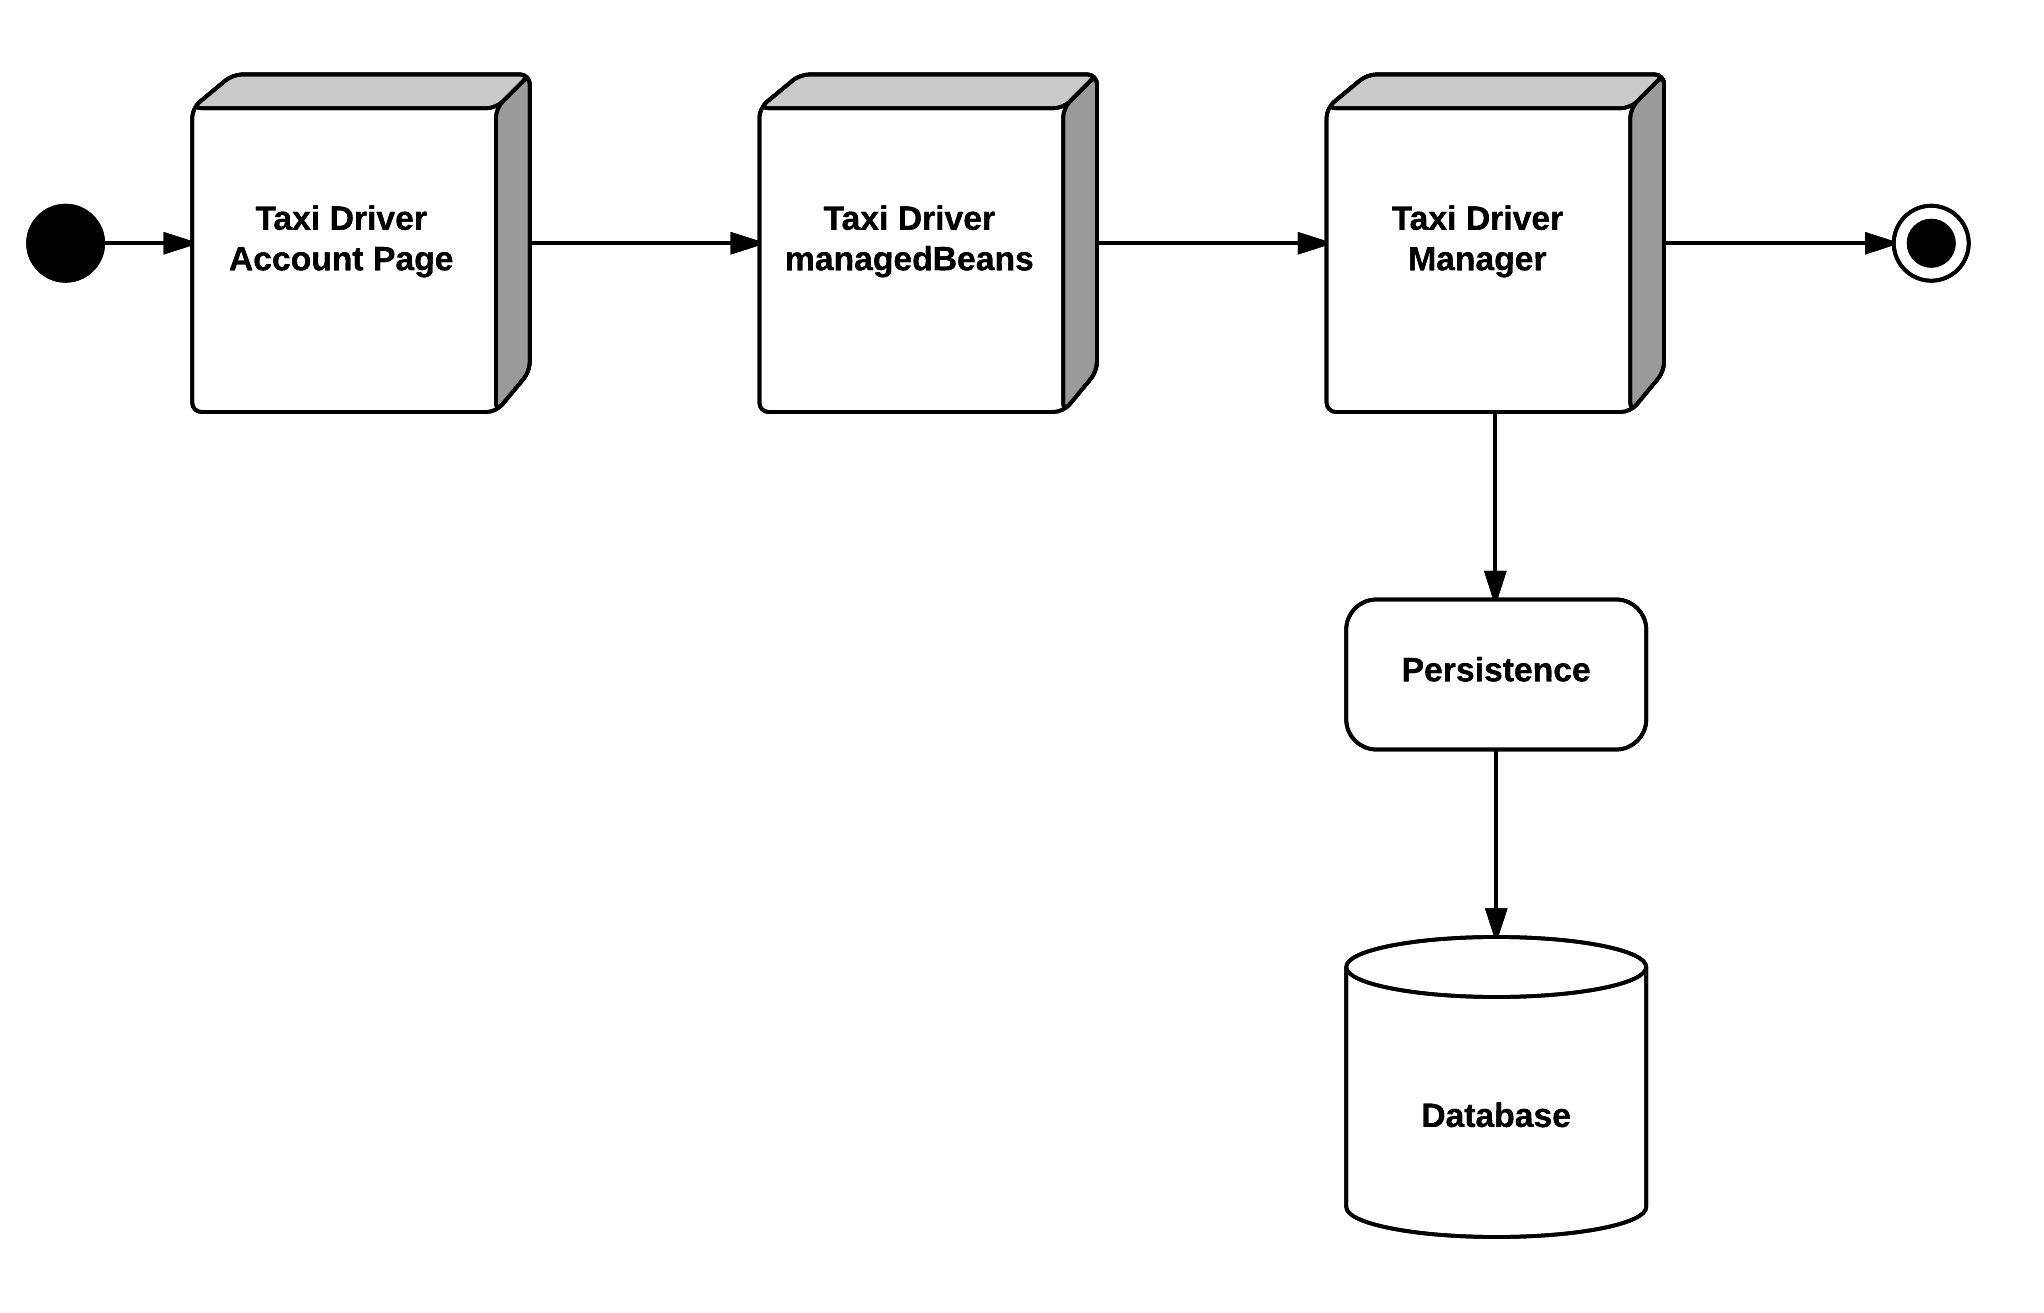
\includegraphics[width=\textwidth]{cpt/img/RuntimeModifyPageTaxidriverView}
	\caption{Runtime Modify Taxi Driver's Account}
	\end{figure}
	\clearpage
	
	\item This diagram represents the components that are involved in the login and registration activities, and their interaction
	\begin{figure}[htbp]
	\centering
	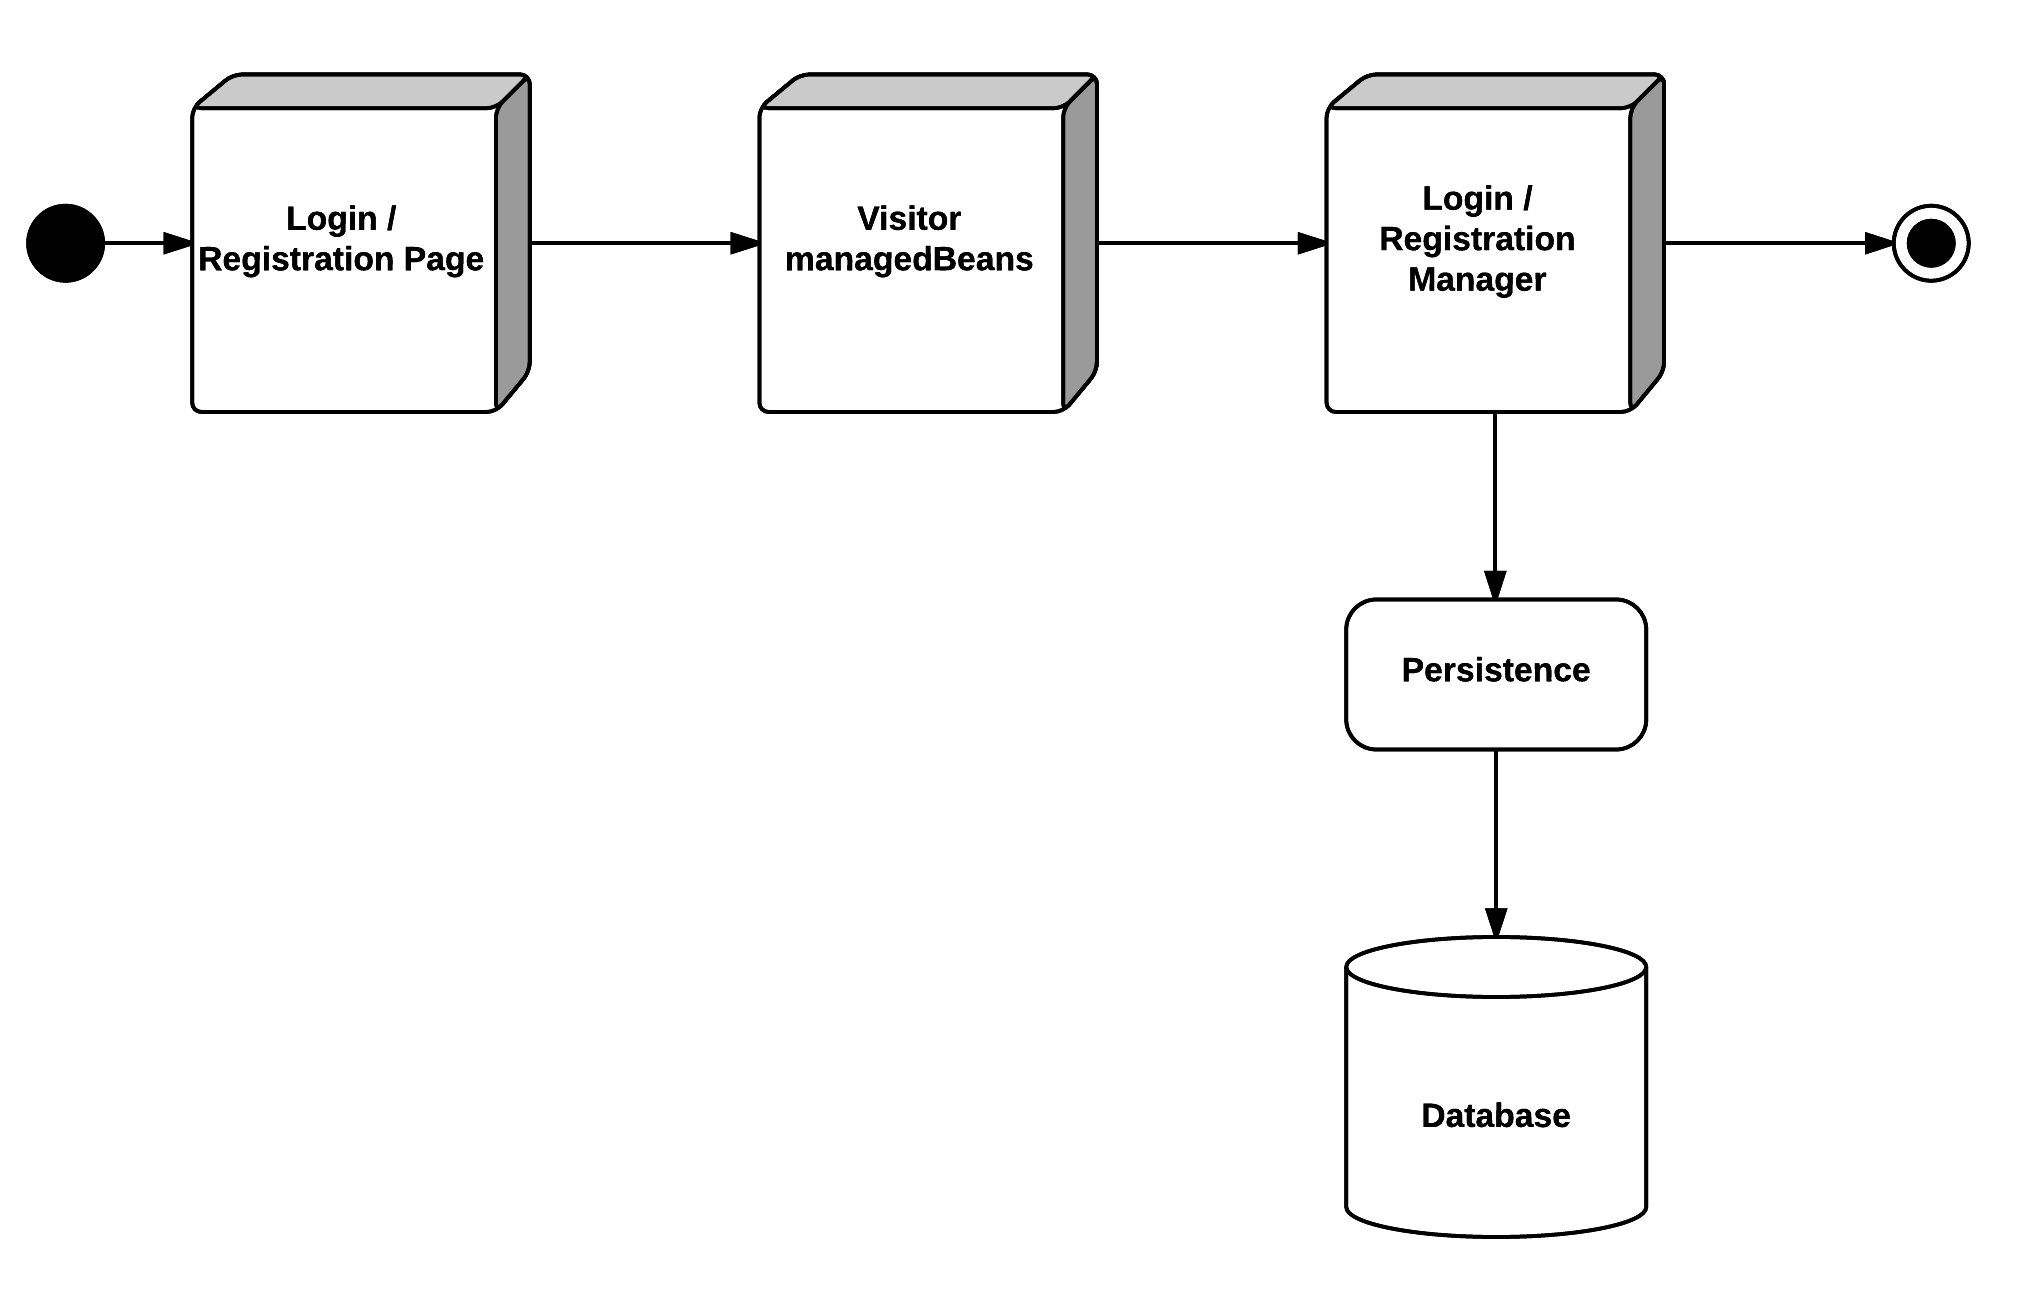
\includegraphics[width=\textwidth]{cpt/img/RuntimeLoginRegisterView}
	\caption{Runtime Login and Registration}
	\end{figure}
	\clearpage
	
	\item This diagram represents the components that are needed during the process of starting a taxi ride, and their interaction
	\begin{figure}[htbp]
	\centering
	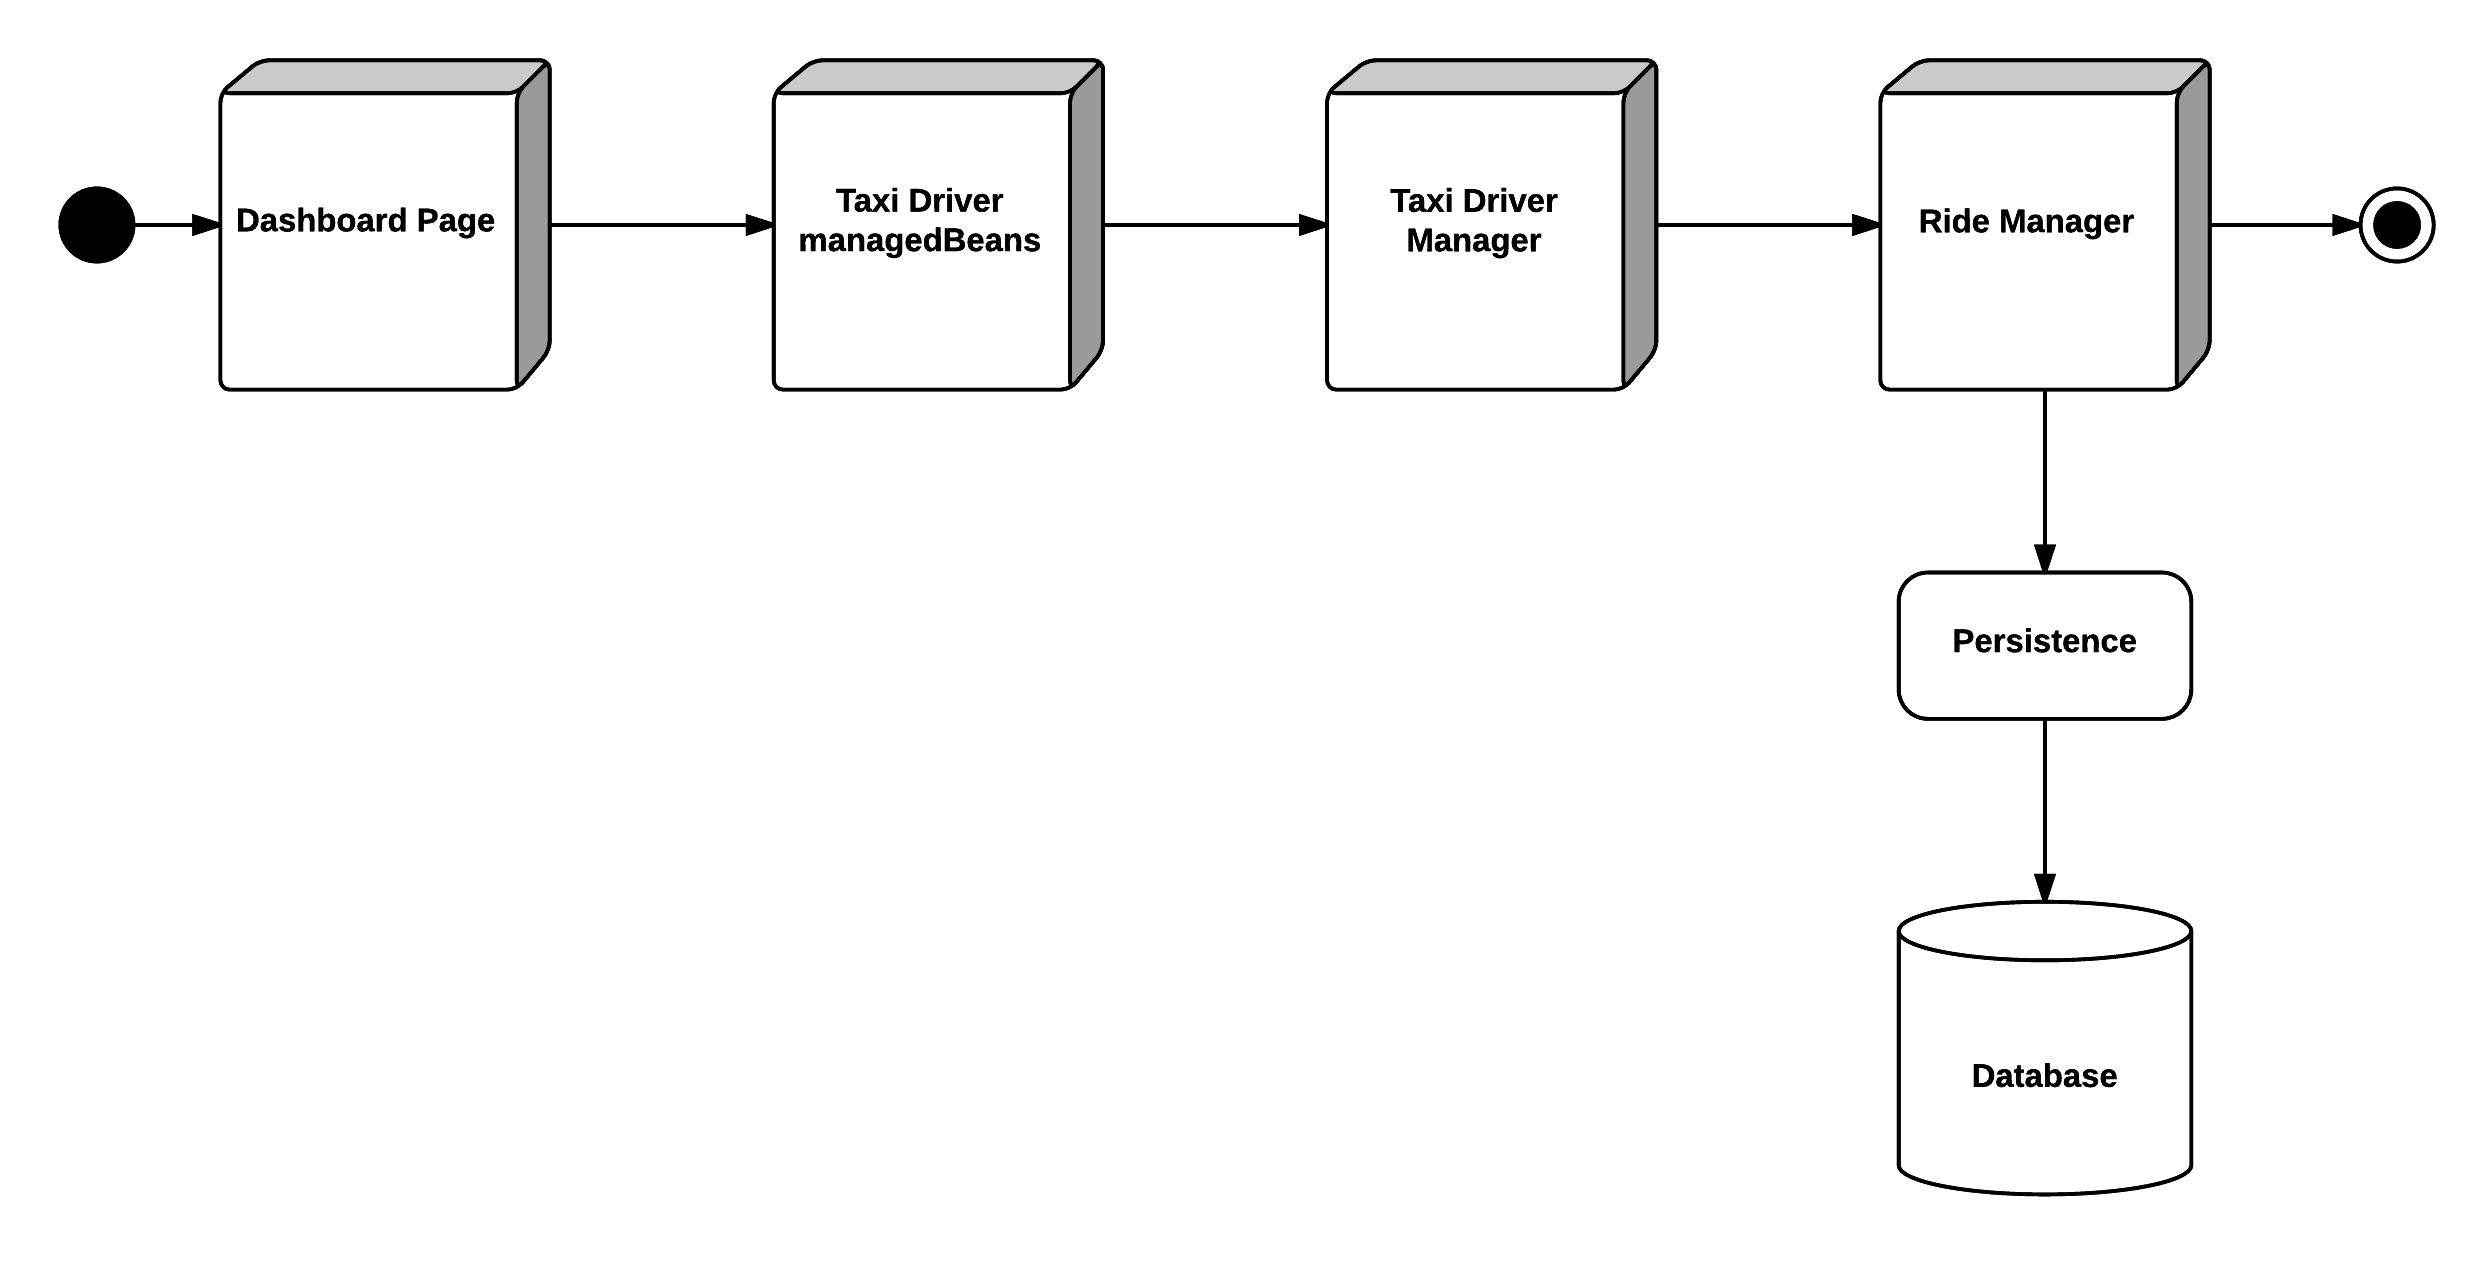
\includegraphics[width=\textwidth]{cpt/img/RuntimeStartTaxiRideView}
	\caption{Runtime start Taxi Ride}
	\end{figure}
	\clearpage
	
	\item This diagram represents the components that are involved in the process of showing the summary of the ride to the taxi driver and their interaction
	\begin{figure}[htbp]
	\centering
	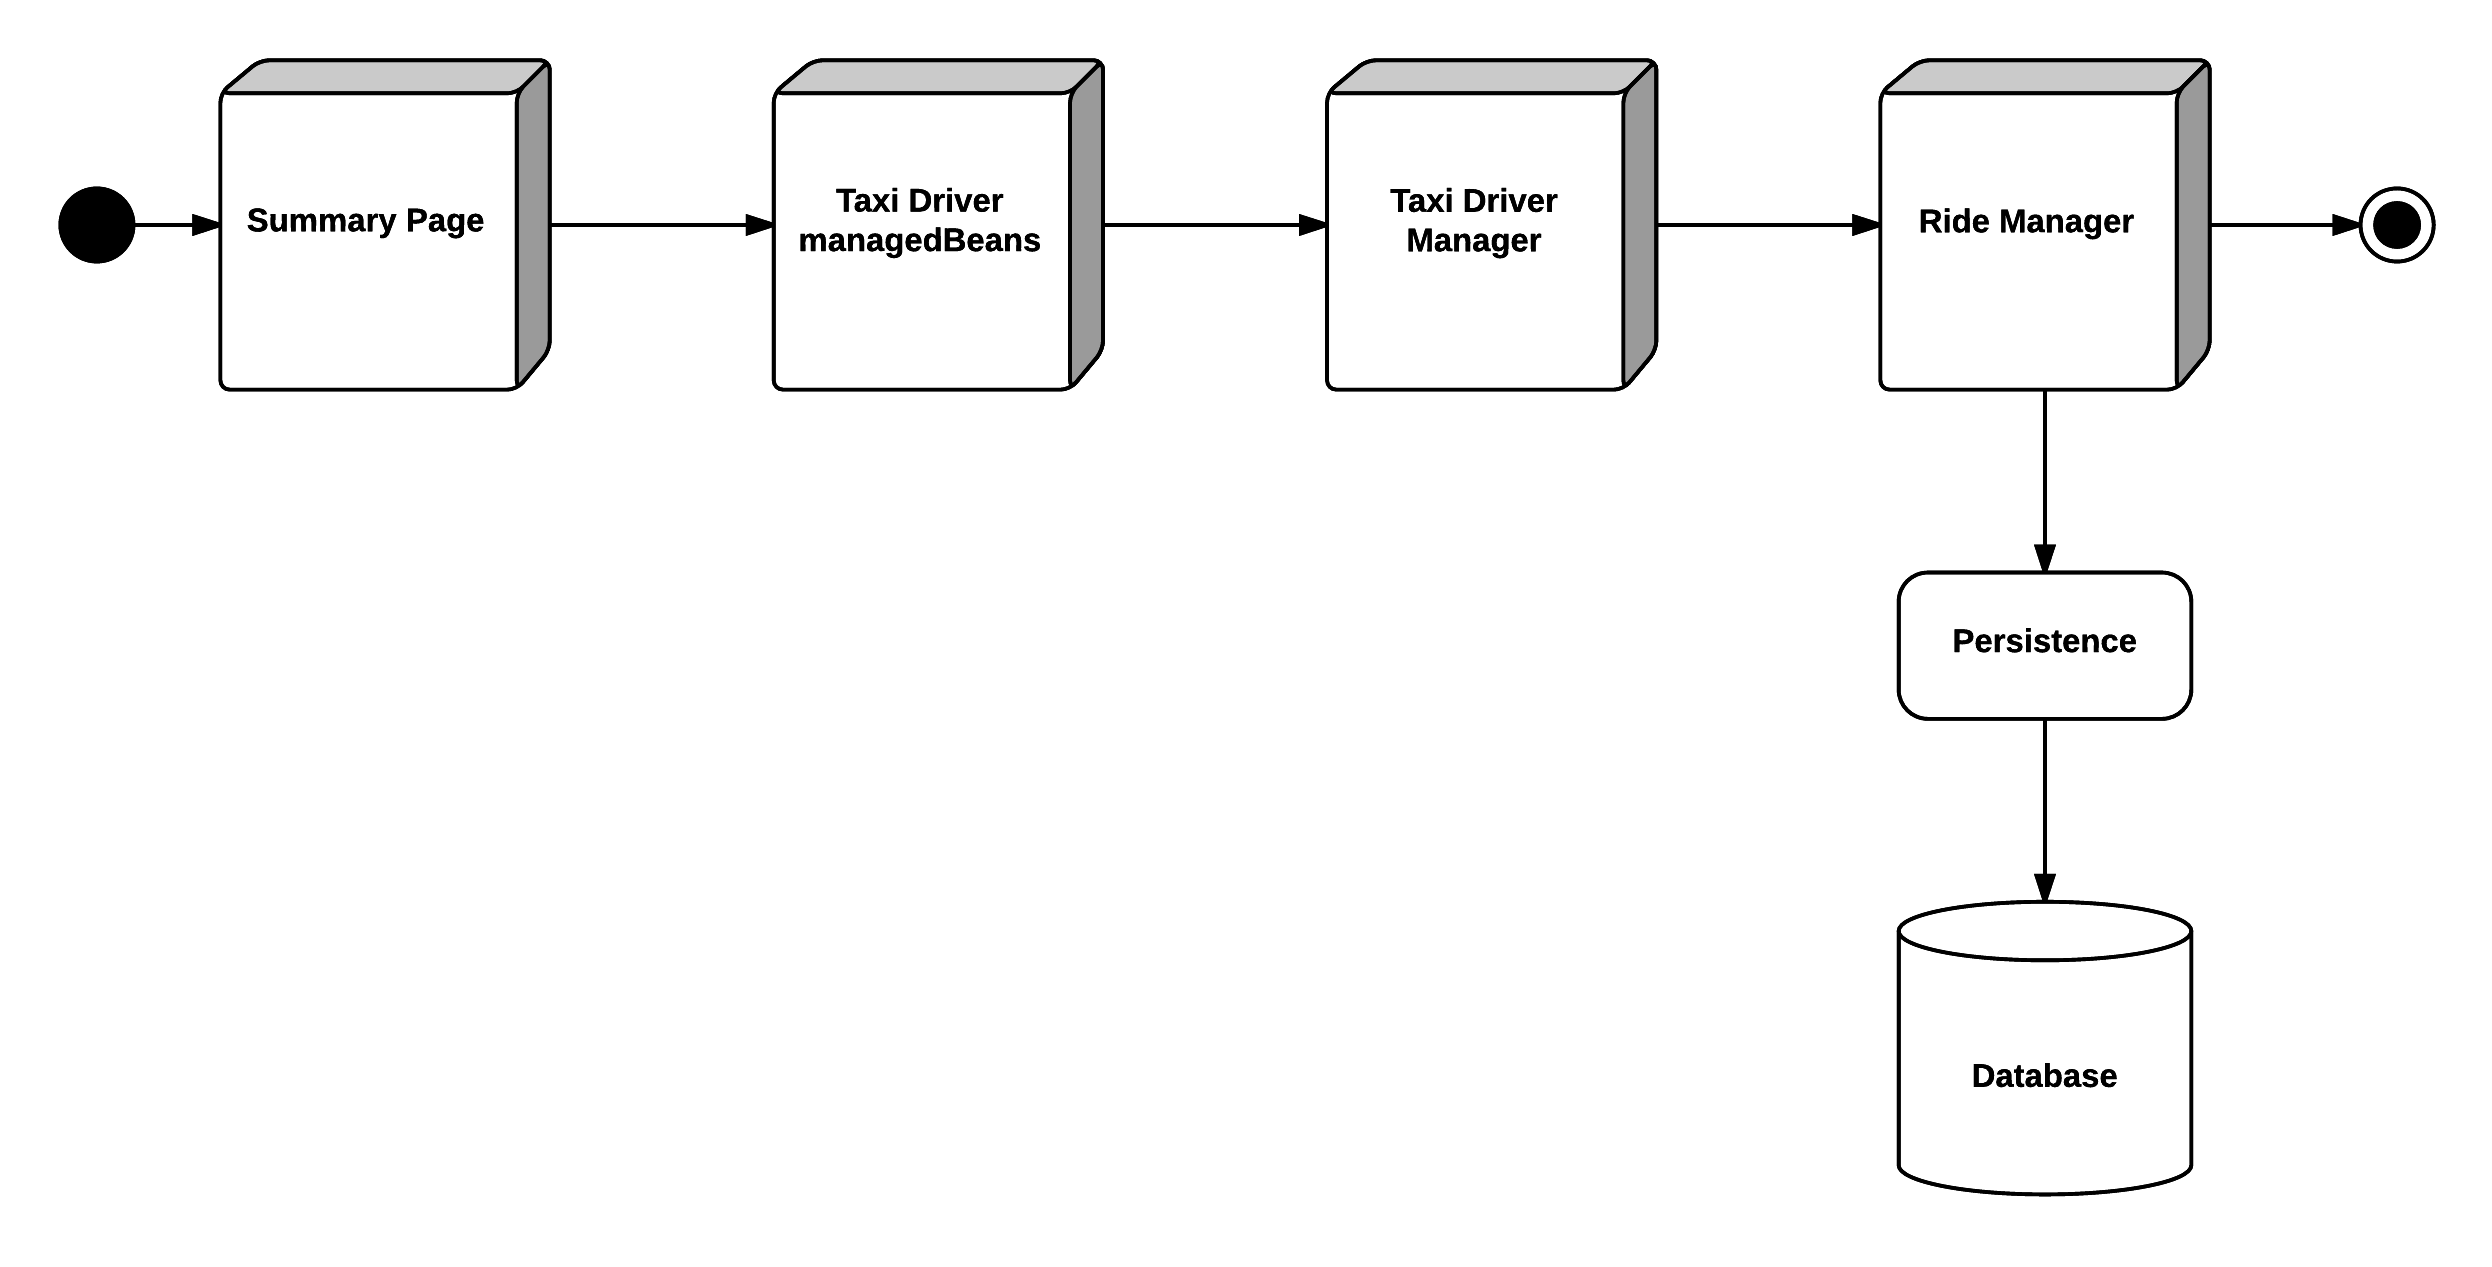
\includegraphics[width=\textwidth]{cpt/img/RuntimeSummaryView}
	\caption{Runtime Summary}
	\end{figure}
	\clearpage

\end{itemize}

\section{Component Interfaces}
Here are identified some functions offered by the Beans of the Business Tier:

\subsubsection{Visitor Manager}
The Visitor Manager should expose some methods like:
\begin{itemize}
	\item \textit{createNewUser} to add a new user to the database 
	\item \textit{verifyLogin} and \textit{verifyRegistration} to check if the information provided by the user in the Login or Registration Pages are correct
\end{itemize}

\begin{figure}[htbp]
\centering
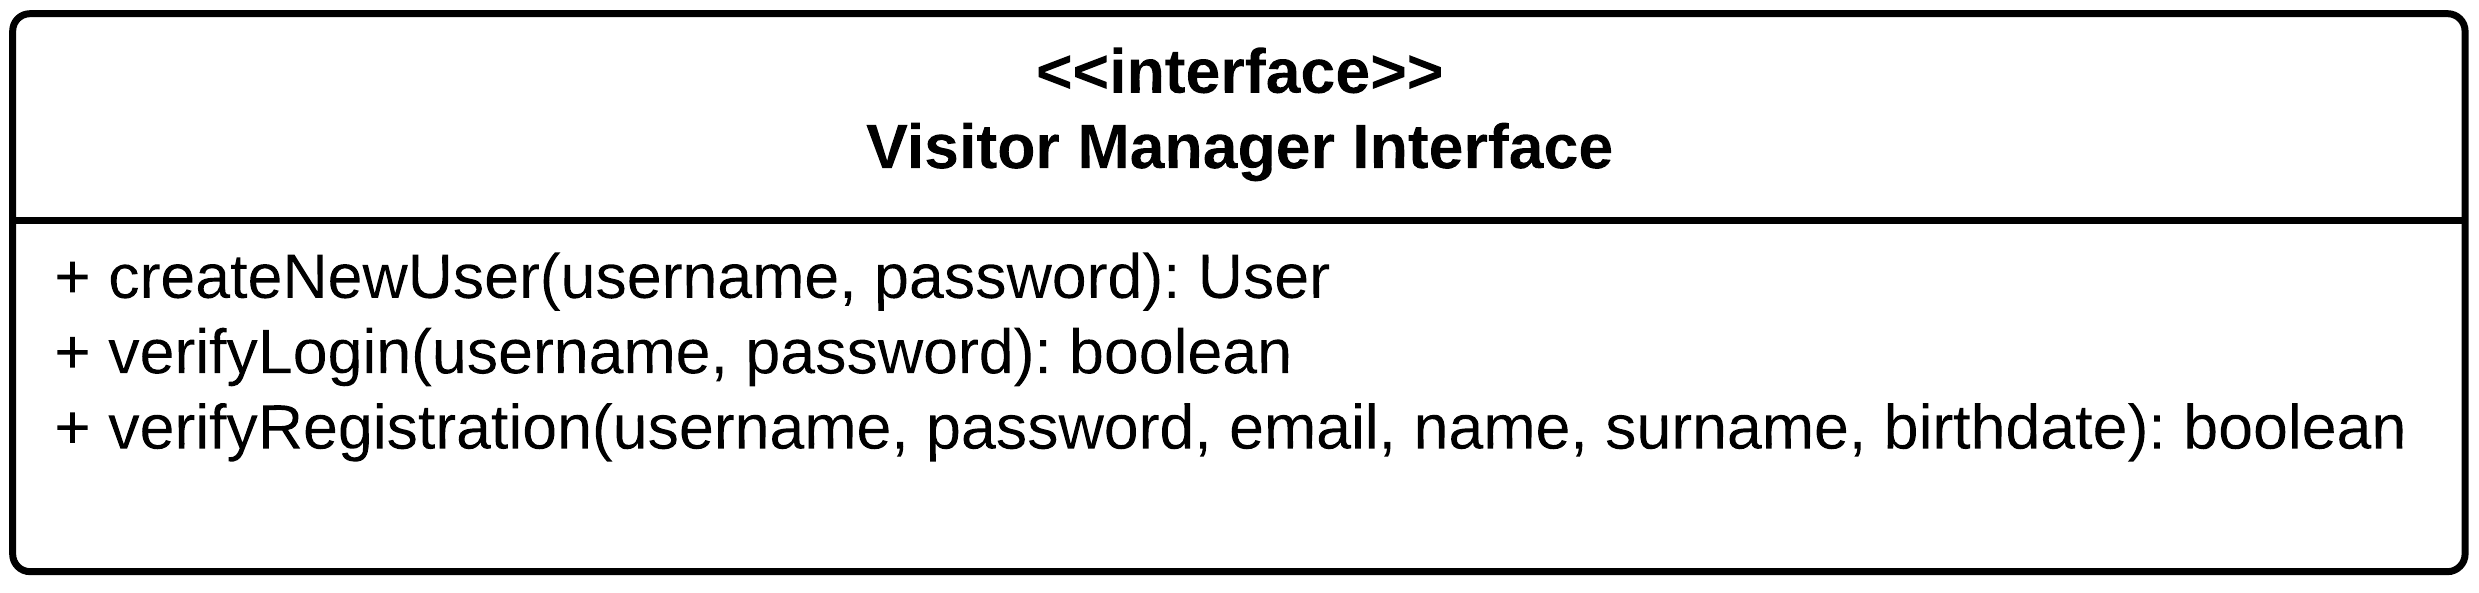
\includegraphics[width=\textwidth]{cpt/img/ComponentInterfacesVisitorManagerInterface}
\caption{Visitor Manager Interface}
\end{figure}
\clearpage

\subsubsection{Passenger Manager}
The Passenger Manager should expose some methods like:
\begin{itemize}
	\item \textit{getPassengerInformation} to retrieve all the information about a certain passenger stored in the database
	\item \textit{getPassengerLocation} to retrieve the passenger position from it?s smartphone GPS
	\item \textit{getPassengerState} to obtain the current state of the passenger
	\item \textit{setPassengerState} to modify the current state of the passenger
	\item \textit{updatePassengerInformation} to update the information about a passenger stored into the database
\end{itemize}

\begin{figure}[htbp]
\centering
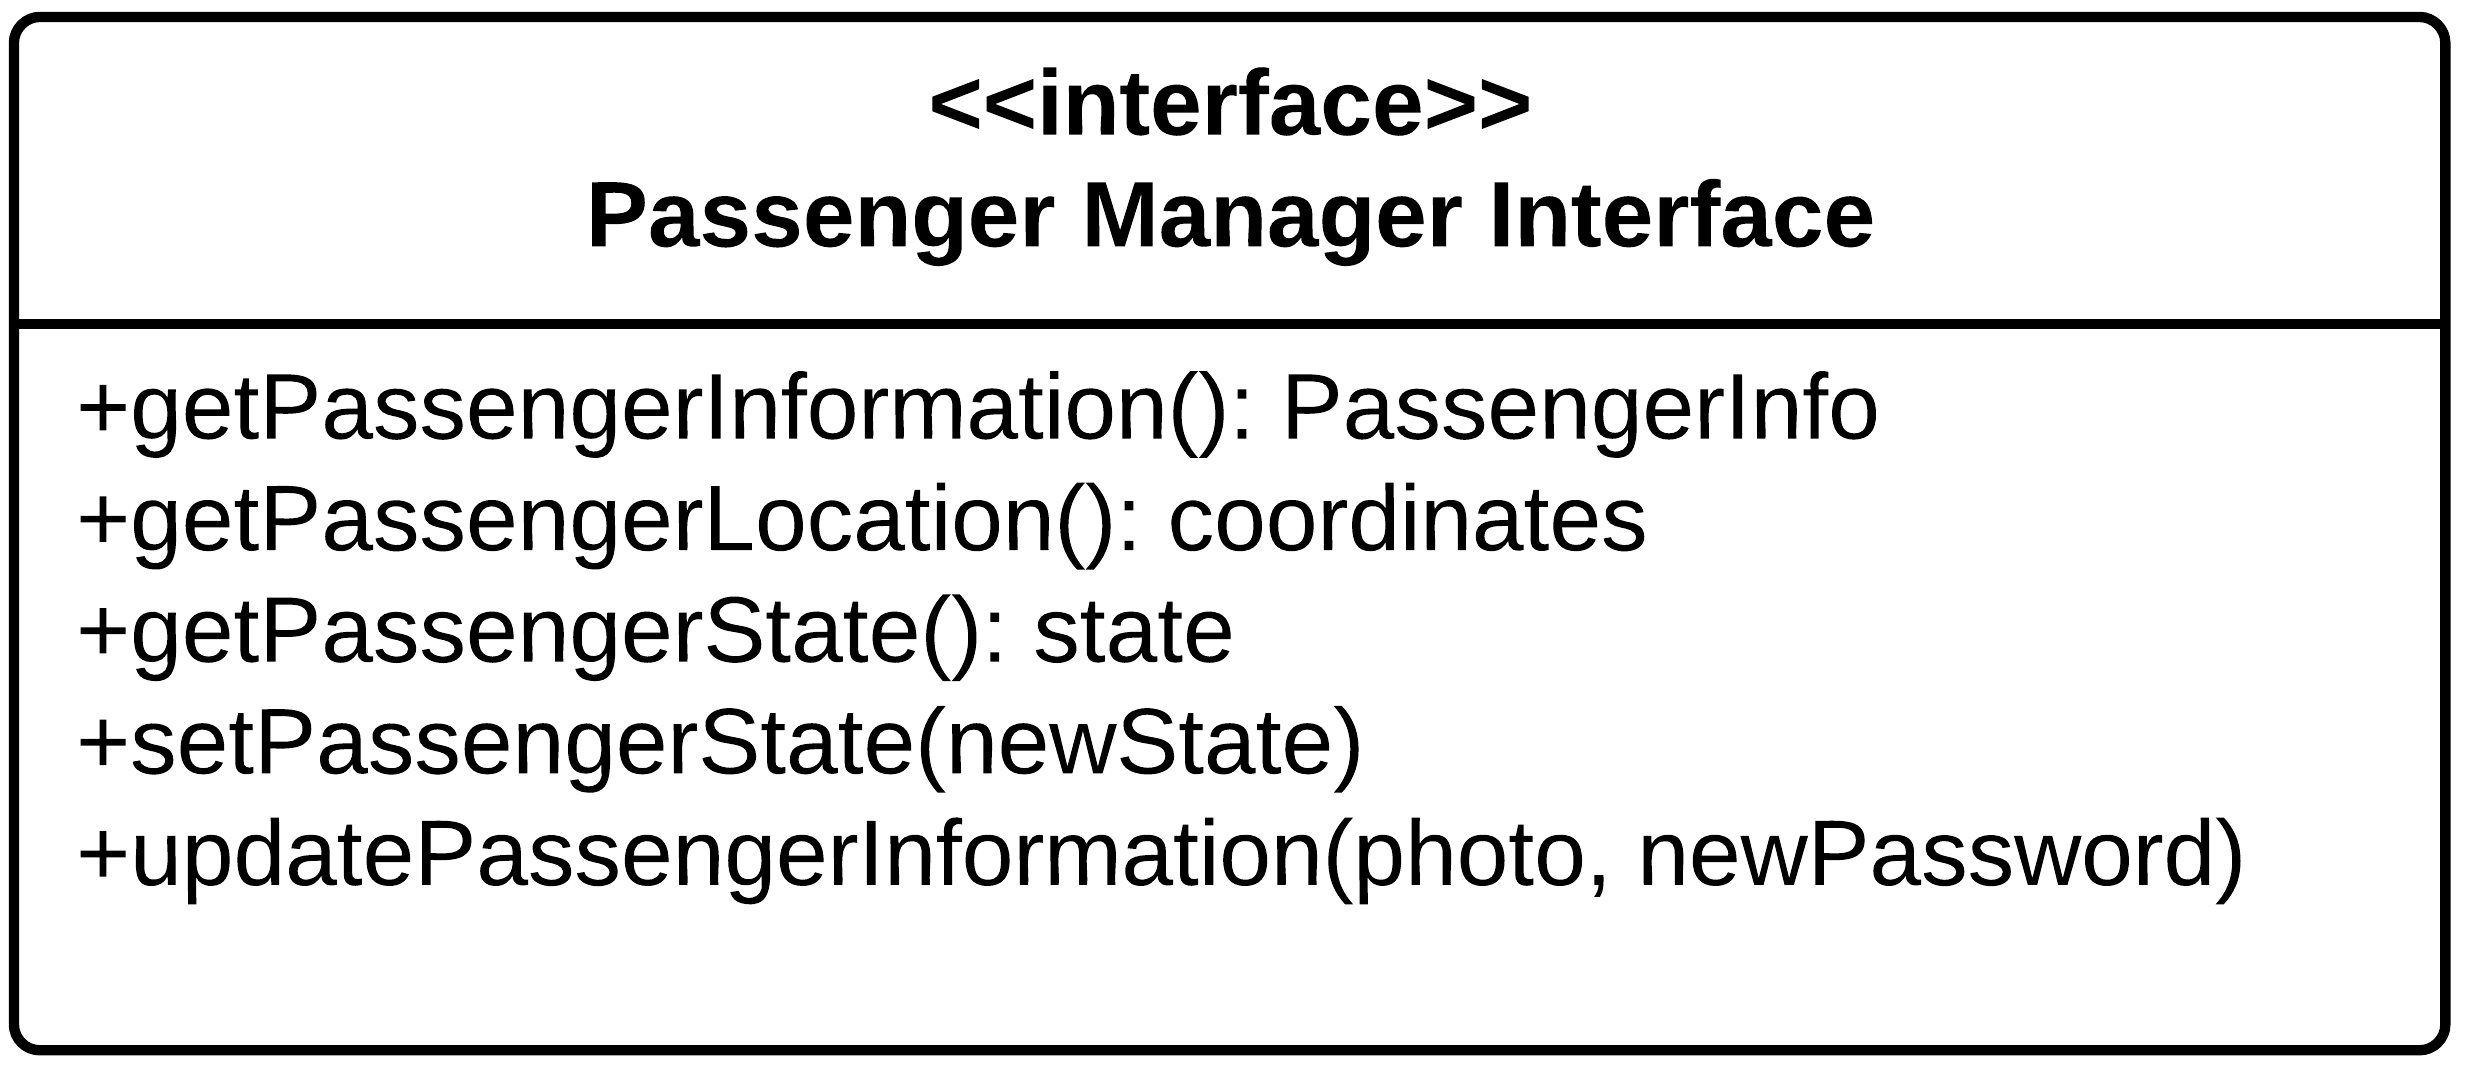
\includegraphics[width=\textwidth]{cpt/img/ComponentInterfacesPassengerManagerInterface}
\caption{Passenger Manager Interface}
\end{figure}
\clearpage

\subsubsection{Taxi Driver Manager}
The Taxi Driver Manager should expose some methods like:
\begin{itemize}
	\item \textit{getTaxiDriverInformation} to retrieve all the needed information about a taxi driver stored into the database
	\item \textit{getTaxiDriverLocation} to retrieve the taxi driver position from it?s GPS device
	\item \textit{updateTaxiDriverInformation} to update the information about a taxi driver stored into the database
	\item \textit{checkTaxiDriverAvailability} to check the current status of the taxi driver
\end{itemize}

\begin{figure}[htbp]
\centering
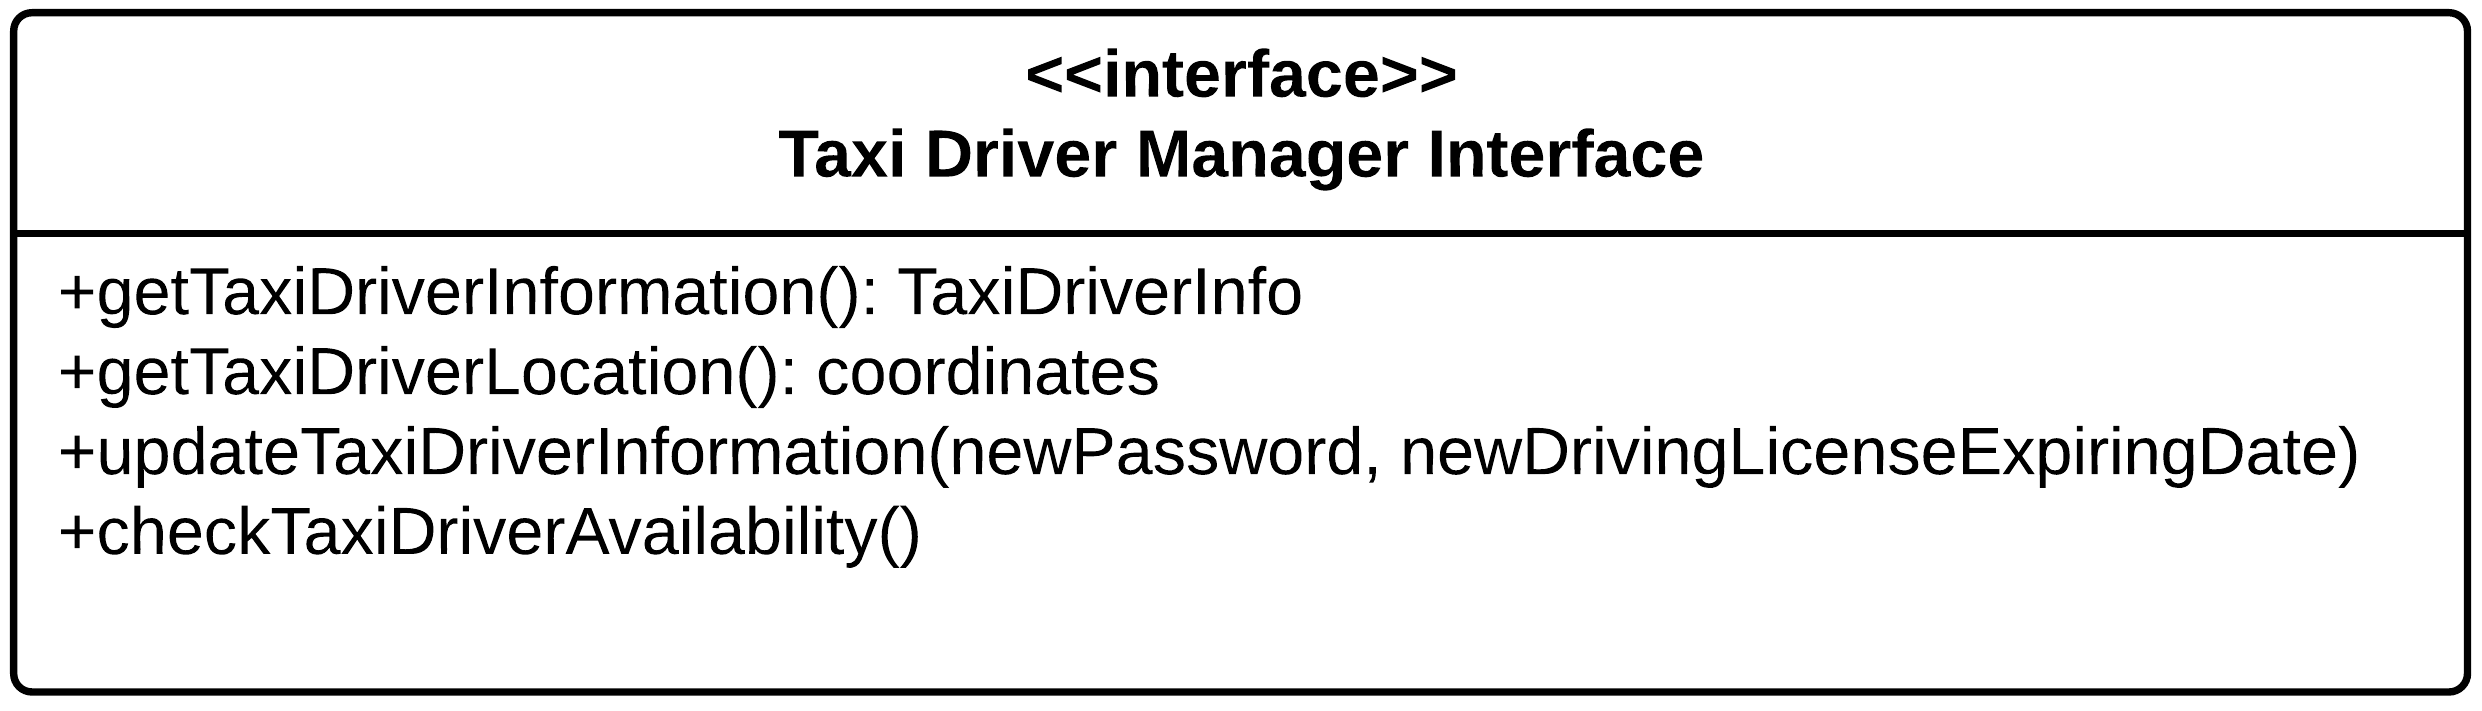
\includegraphics[width=\textwidth]{cpt/img/ComponentInterfacesTaxiDriverManagerInterface}
\caption{Taxi Driver Manager Interface}
\end{figure}
\clearpage

\subsubsection{Developer Manager}
The Developer Manager should expose some methods like:
\begin{itemize}
	\item \textit{updateDeveloperInformation} to update the information about a developer stored into the database
	\item \textit{codeInspector} to see the whole system's code
	\item \textit{addFeature} to write code
	\item \textit{updateCode} to update the whole system's code
\end{itemize}

\begin{figure}[htbp]
\centering
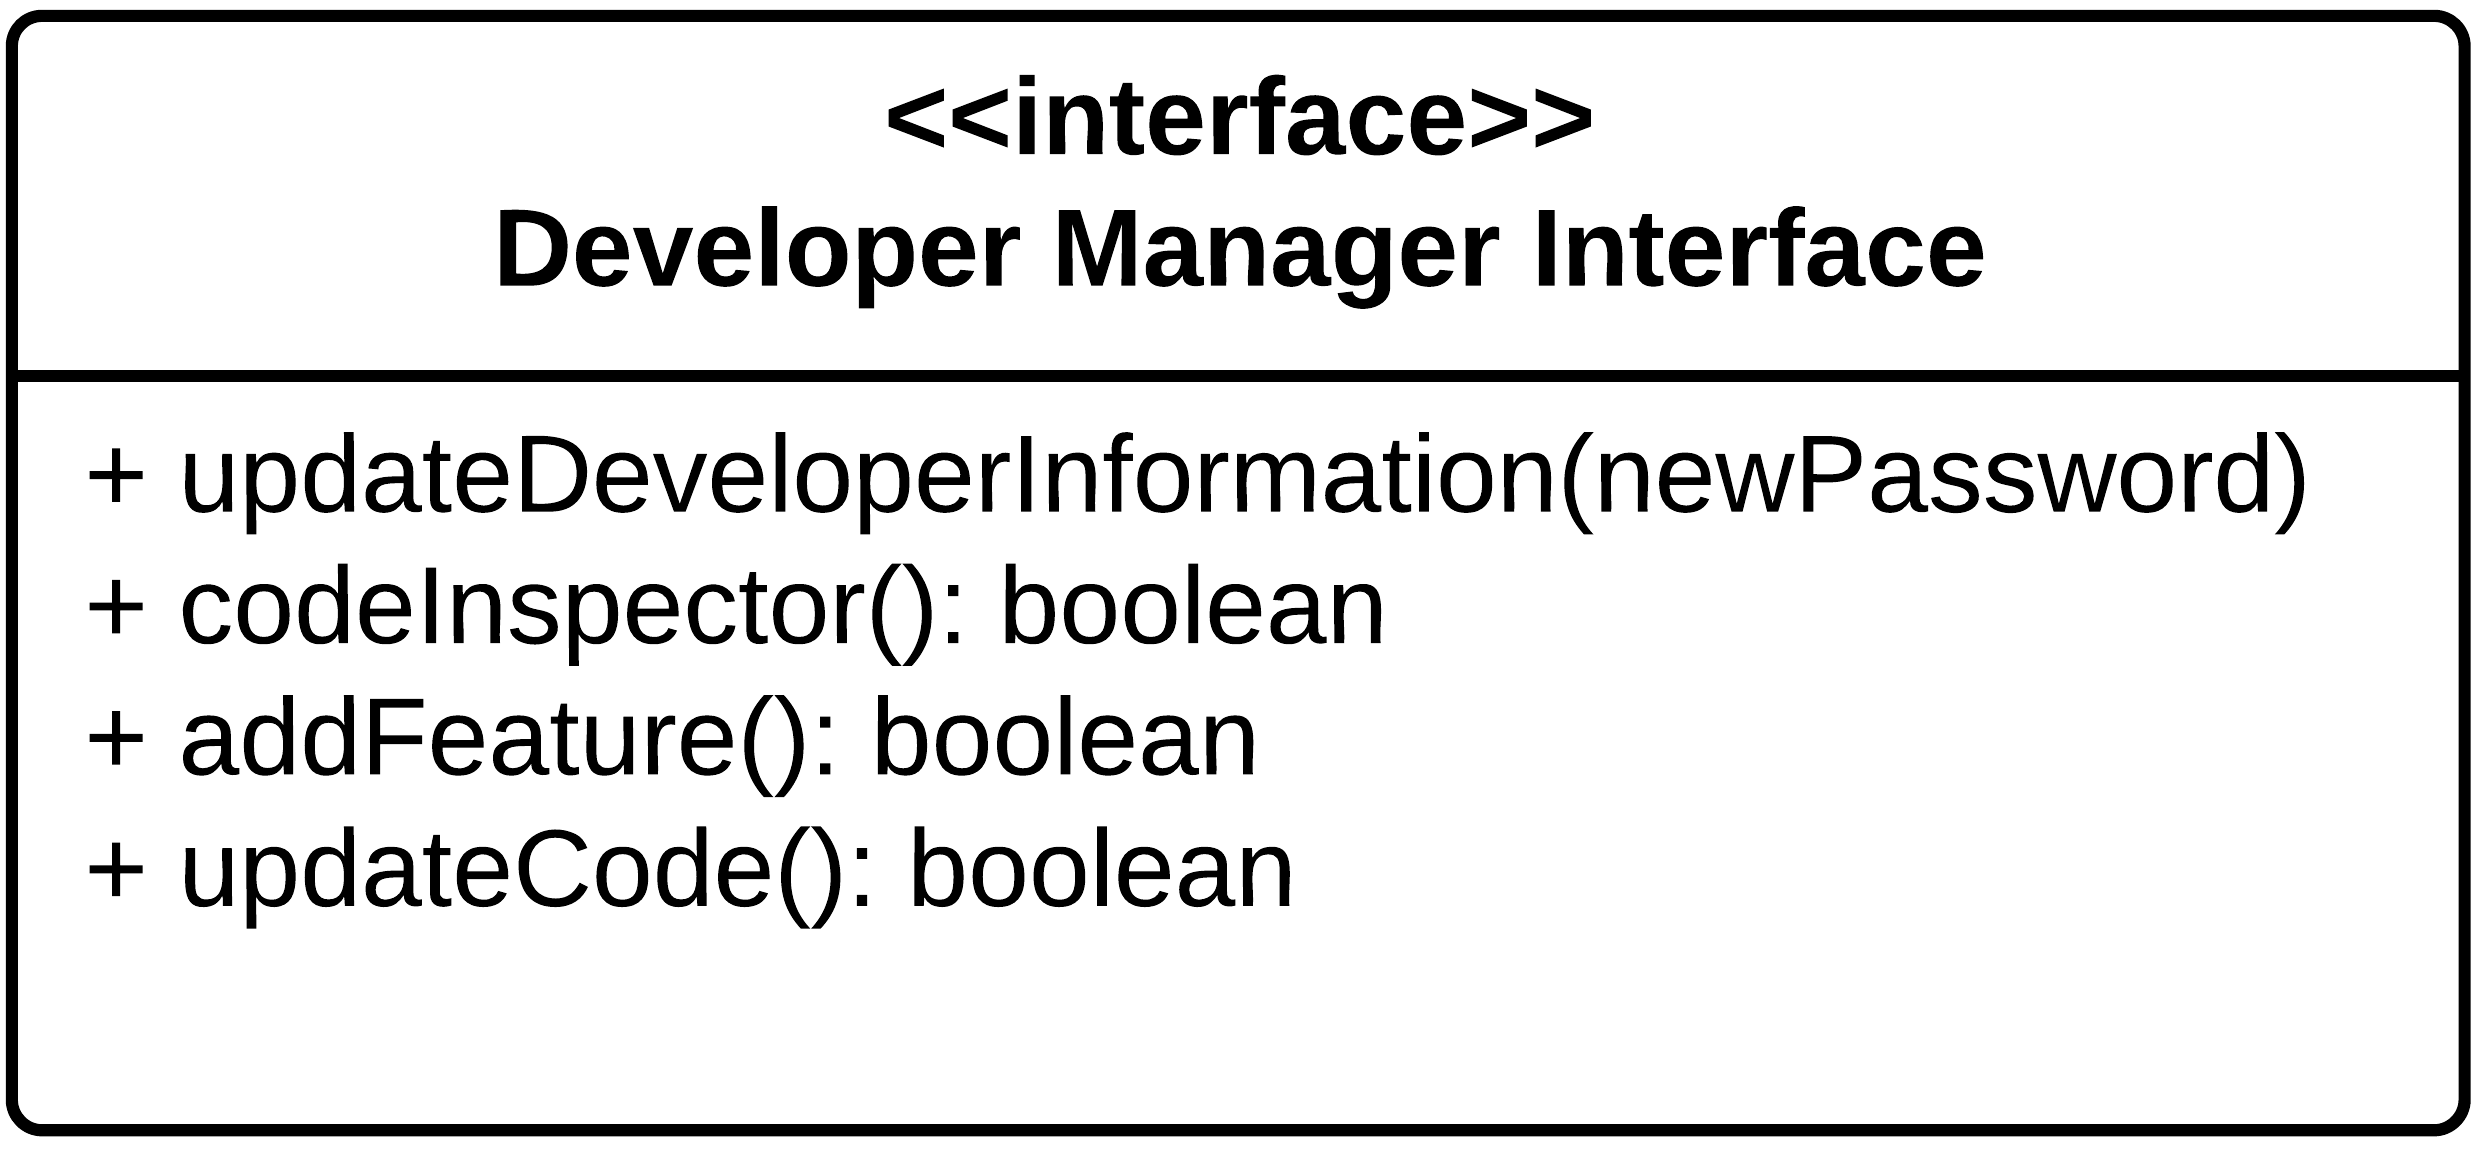
\includegraphics[width=\textwidth]{cpt/img/ComponentInterfacesDeveloperManagerInterface}
\caption{Developer Manager Interface}
\end{figure}
\clearpage

\subsubsection{Calls Manager}
The Calls Manager should expose some methods like:
\begin{itemize}
	\item \textit{createNewCall} to elaborate an incoming request or reservation from the ManagedBeans of the web tier
	\item \textit{updateCall} to modify the status of a pending call
	\item \textit{searchForRide} to start the research of a feasible ride that fulfills the client?s request / reservation (origin, destination, sharing) and thus the research of an available taxi driver
\end{itemize}

\begin{figure}[htbp]
\centering
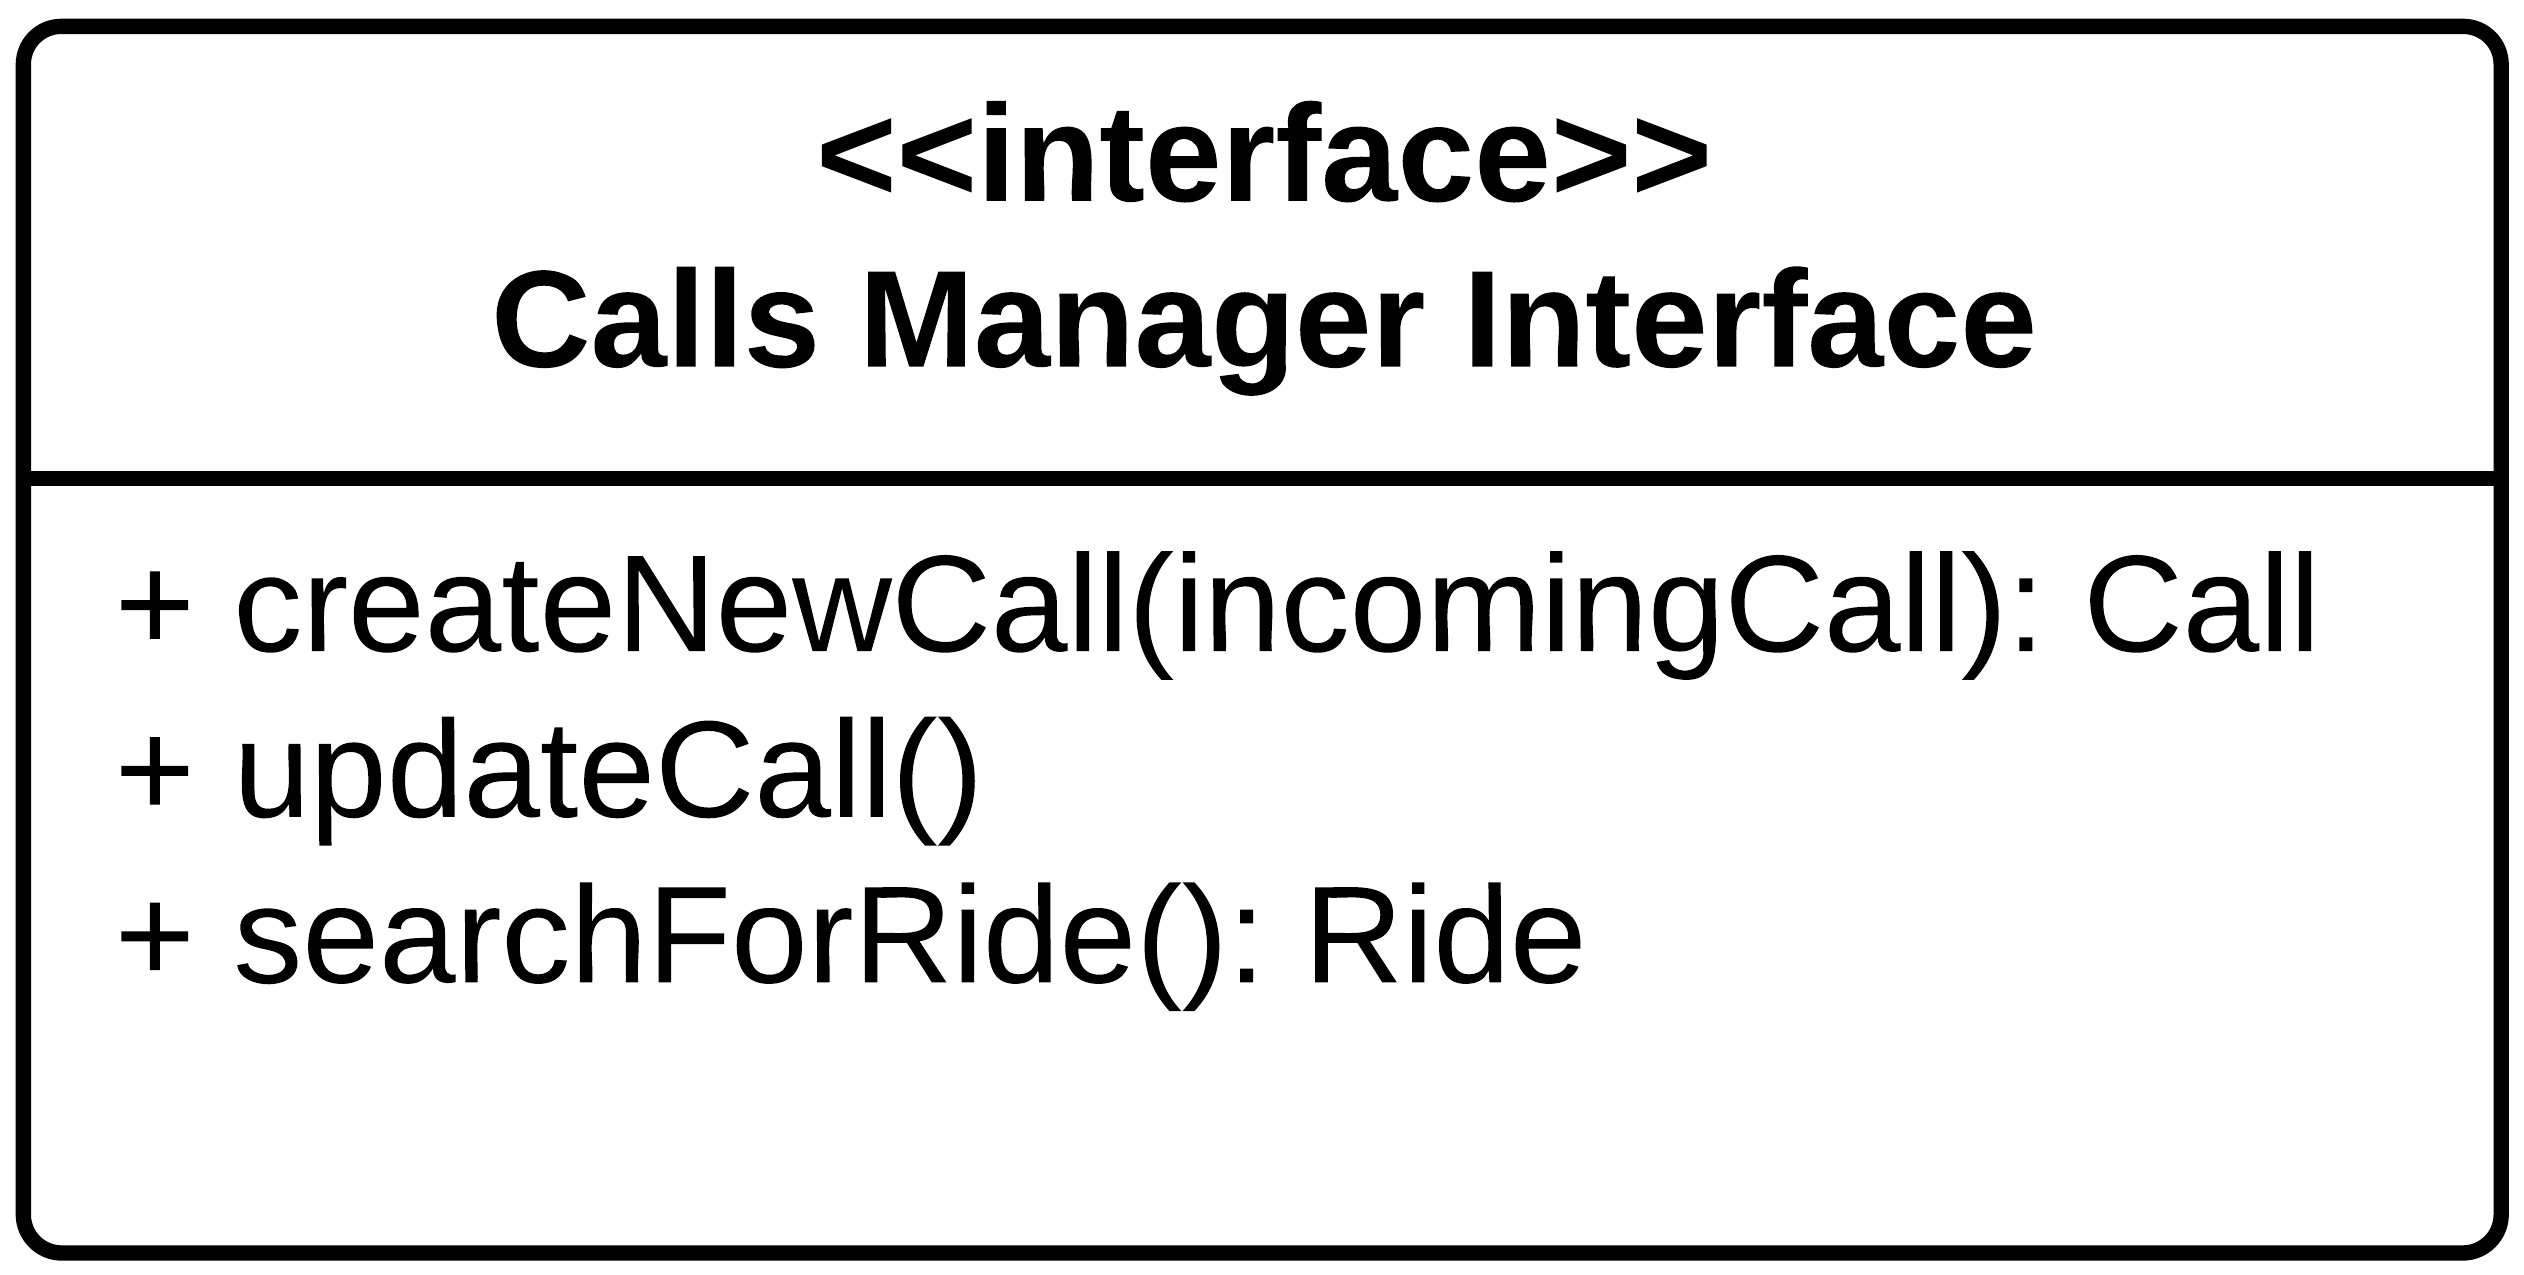
\includegraphics[width=\textwidth]{cpt/img/ComponentInterfacesCallManagerInterface}
\caption{Calls Manager Interface}
\end{figure}
\clearpage

\subsubsection{Ride Manager}
The Ride Manager should expose some methods like:
\begin{itemize}
	\item \textit{createNewRoute} to receive the information about the selected ride and elaborate the optimal route for the taxi driver
	\item \textit{collectRideData} to collect and store all the useful data about the ride (i.e. durations, number of passengers, total fee, fee per passenger, taxi driver, length)
	\item \textit{exportRideData} to share collected data with other component or systems
\end{itemize}

\begin{figure}[htbp]
\centering
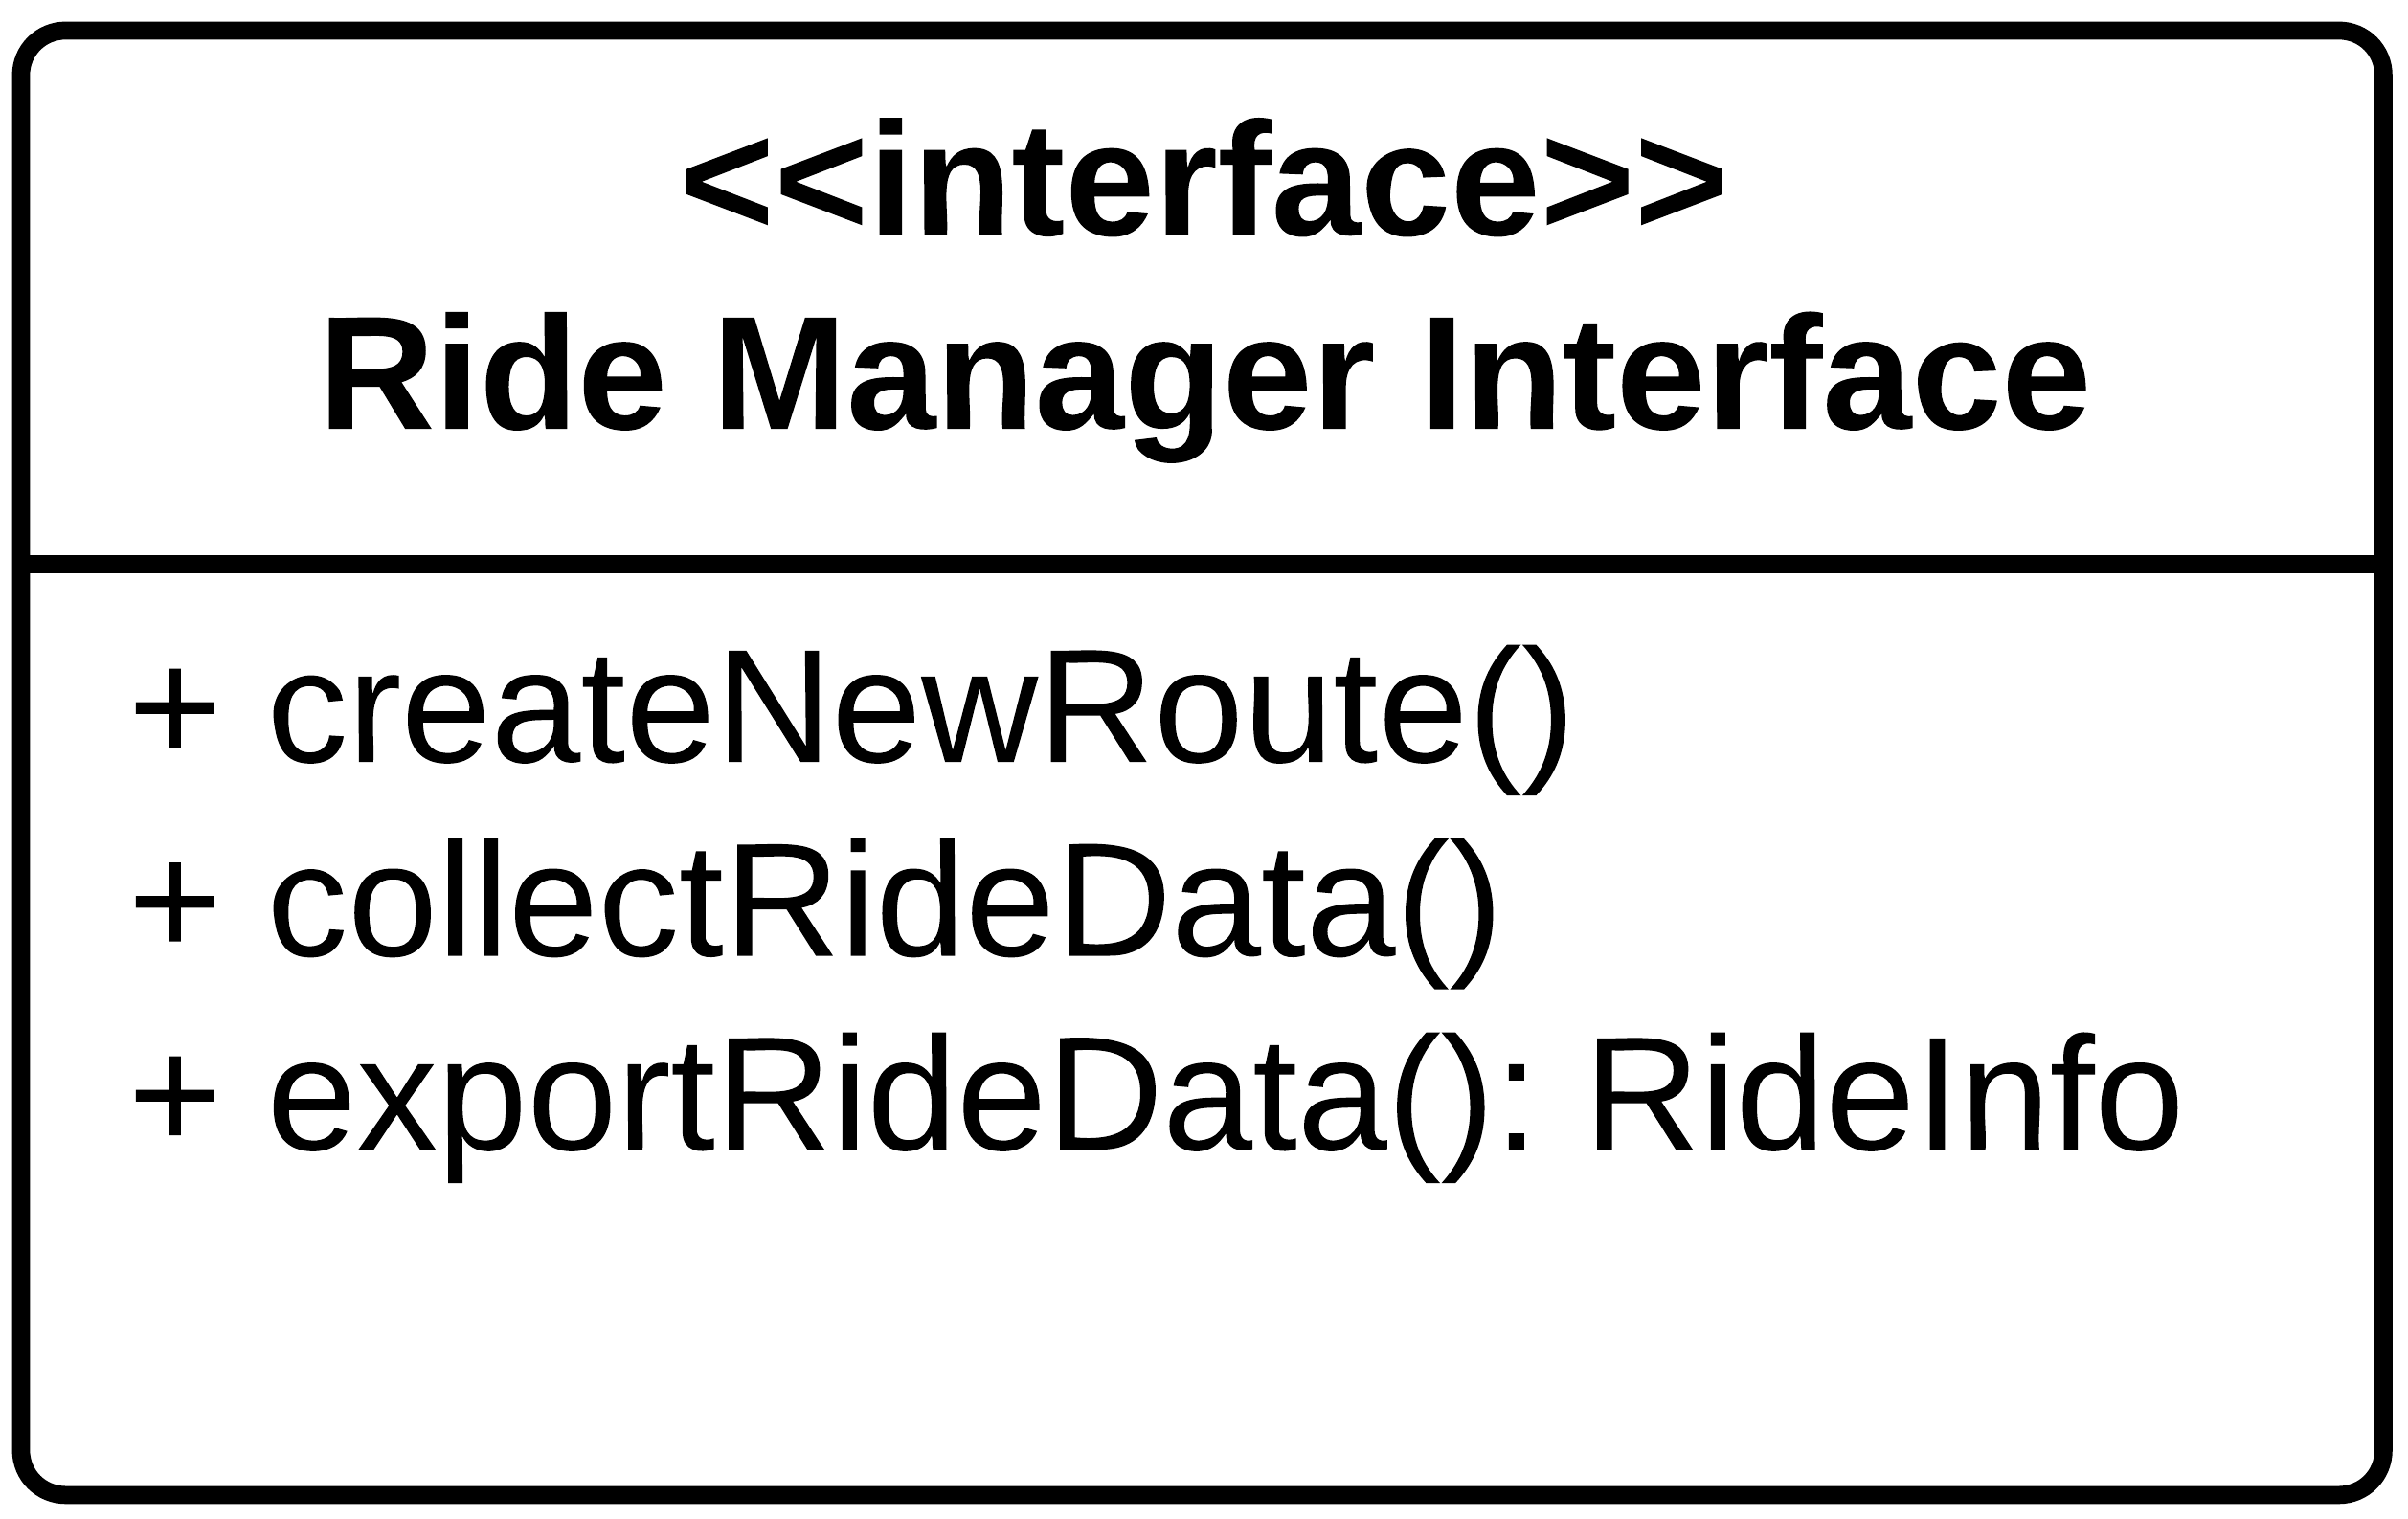
\includegraphics[width=\textwidth]{cpt/img/ComponentInterfacesRideManagerInterface}
\caption{Ride Manager Interface}
\end{figure}
\clearpage

\section{Selected Architectural Styles and Patterns}
During the developing of this document and the construction of the system we have focused on keeping the architecture and the general behavior of the system as simple as possible, trying to adapt everything to the architecture of Java EE which is a very good starting point for a system like ours. In our mind this initial simplicity and modularity leaves the right amount of space for further improvements and strengthening of the system. Moreover, given the nature of the system (a taxi sharing application) we think that this 4-tier architecture that relies upon the Model - View - Controller pattern is the one that most fits the requirements and grants optimal performances in terms of reliability, availability and performances of the system.